%--------------------------------------------------------------------%
%
% Berkas utama templat LaTeX.
%
% author Petra Barus, Peb Ruswono Aryan, Faris Rizki Ekananda
%
%--------------------------------------------------------------------%
%
% Berkas ini berisi struktur utama dokumen LaTeX yang akan dibuat.
%
%--------------------------------------------------------------------%

\documentclass[bahasa, 12pt, a4paper, onecolumn, oneside, final]{report}

%-------------------------------------------------------------------%
%
% Konfigurasi dokumen LaTeX untuk laporan tesis IF ITB
%
% @author Petra Novandi
%
%-------------------------------------------------------------------%
%
% Berkas asli berasal dari Steven Lolong
%
%-------------------------------------------------------------------%

% Ukuran kertas
\special{papersize=210mm,297mm}

% Setting margin
\usepackage[top=3cm,bottom=3cm,left=4cm,right=3cm]{geometry}

\usepackage{mathptmx}
\usepackage{mathtools}

% Judul bahasa Indonesia
\usepackage[bahasa]{babel}

% Format citation
\usepackage[style=apa,backend=biber]{biblatex}

% \setmainlanguage{bahasa}
% \setotherlanguage{english}
\usepackage{array}
\usepackage{algorithm}
\usepackage{algpseudocode}
\usepackage{booktabs}
\usepackage[raggedrightboxes]{ragged2e}
\usepackage[utf8]{inputenc}
\usepackage{amsmath, xparse}
\usepackage{graphicx}
\usepackage{adjustbox}
\usepackage{titling}
\usepackage{blindtext}
\usepackage{sectsty}
\usepackage{chngcntr}
\usepackage{etoolbox}
\usepackage[hidelinks]{hyperref}       % Package untuk link di daftar isi.
\usepackage{titlesec}       % Package Format judul
\usepackage{titletoc}       % Package Format judul di toc
\usepackage{tocbibind}      % Package untuk masukkan toc, lot, lof ke Daftar Isi
\usepackage{scrwfile}       % Package untuk membuat Daftar Lampiran dari toc
\usepackage{parskip}
\usepackage{afterpage}
\usepackage{relsize}
\usepackage{float}
\usepackage{longtable} % Package untuk table multipage
\usepackage{multirow}
\usepackage{caption}
\usepackage[table, svgnames, xcdraw]{xcolor} % Package untuk table color
\usepackage{soul}
\usepackage{setspace} % untuk set baseline ditengah2
\usepackage{tabto}
\usepackage{listings}
\usepackage{lscape}
\usepackage[normalem]{ulem}
\useunder{\uline}{\ul}{}
\usepackage{color}
\usepackage{spverbatim}

\graphicspath{{resources/}}   % letak direktori penyimpanan gambar

\setlength{\LTcapwidth}{\textwidth}

\captionsetup{font=normalsize,justification=centering,margin=1cm}

\newenvironment{tabs}[1]
 {\flushleft\TabPositions{#1}}
 {\endflushleft}

%  Set kedalaman ToC
 \setcounter{tocdepth}{3}

% Setting daftar lampiran
\newcommand*{\lopname}{DAFTAR LAMPIRAN}
\TOCclone[\lopname]{toc}{atoc}
\addtocontents{atoc}{\protect\value{tocdepth}=-1}
\newcommand\listofappendices{
  \cleardoublepage
  \phantomsection
  \listofatoc
  \addcontentsline{toc}{chapter}{\lopname}
}

\newcommand*\savedtocdepth{}
\AtBeginDocument{%
  \edef\savedtocdepth{\the\value{tocdepth}}%
}

\let\originalappendix\appendix
\renewcommand\appendix{%
  \originalappendix
  \cleardoublepage
  \addtocontents{toc}{\protect\value{tocdepth}=-1}%
  \addtocontents{atoc}{\protect\value{tocdepth}=\savedtocdepth}%

  \titlecontents{chapter}
    [0pt]
    {\bfseries}
    {Lampiran \thecontentslabel.\quad}
    {}
    {\hfill\contentspage}

  \titleformat{\chapter}[block]
    {\bfseries}
    {\chaptertitlename\ \thechapter.\quad}{0pt}
    {\bfseries}
}

% Perkecil titik pada toc
\makeatletter
\renewcommand{\@dotsep}{1} 
\makeatother

% Setel title pada chapter-chapter di toc, lof, lot
\titlecontents{chapter}
  [0pt]
  {\bfseries}
  {\MakeUppercase{Bab} \thecontentslabel\quad\uppercase}
  {}
  {\mdseries\titlerule*[0.35em]{.}\bfseries\contentspage}
\titlecontents{figure}
  [0pt]
  {}
  {Gambar \thecontentslabel.\quad}
  {}
  {\mdseries\titlerule*[0.35em]{.}\bfseries\contentspage}
\titlecontents{table}
  [0pt]
  {}
  {Tabel \thecontentslabel.\quad}
  {}
  {\mdseries\titlerule*[0.35em]{.}\bfseries\contentspage}

% Masukin Daftar Pustaka ke toc
\let\originalprintbibliography\printbibliography
\renewcommand\printbibliography{%
  \phantomsection
  \cleardoublepage
  \originalprintbibliography
  \addcontentsline{toc}{chapter}{\bibname}
}

% Line satu setengah spasi
\renewcommand{\baselinestretch}{1.5}

% Setting judul
\chapterfont{\centering \Large}
\titleformat{\chapter}[display]
  {\Large\centering\bfseries}
  {\chaptertitlename\ \thechapter}{0pt}
    {\Large\bfseries\uppercase}

% Setting nomor pada subbsubsubbab
\setcounter{secnumdepth}{3}

\makeatletter
\renewcommand{\ALG@name}{Algoritma}%
\renewcommand{\algorithmicrequire}{\textbf{Prasyarat:}}
\counterwithin{algorithm}{chapter}
\makeatother

% % Counter untuk figure dan table.
% \counterwithin{figure}{section}
% \counterwithin{table}{section}

% Define blank page
\newcommand*{\blankpage}{\afterpage{\null\newpage}}

% Translate autoref into Indonesian
\renewcommand*{\equationautorefname}{Persamaan}%
\renewcommand*{\footnoteautorefname}{catatan kaki}%
\renewcommand*{\itemautorefname}{item}%
\renewcommand*{\figureautorefname}{Gambar}%
\renewcommand*{\tableautorefname}{Tabel}%
\renewcommand*{\partautorefname}{Bagian}%
\renewcommand*{\appendixautorefname}{Lampiran}%
\renewcommand*{\chapterautorefname}{Bab}%
\renewcommand*{\sectionautorefname}{Subbab}%
\renewcommand*{\subsectionautorefname}{Subsubbab}%
\renewcommand*{\subsubsectionautorefname}{Subsubsubbab}%
\renewcommand*{\paragraphautorefname}{paragraf}%
\renewcommand*{\subparagraphautorefname}{subparagraf}%
\renewcommand*{\FancyVerbLineautorefname}{garis}%
\renewcommand*{\theoremautorefname}{Teorema}%
\renewcommand*{\pageautorefname}{halaman}%
\renewcommand\thealgorithm{\thechapter.\arabic{algorithm}} 


%%% biblatex hyperlink cite author and year
% ref: https://tex.stackexchange.com/questions/15951/hyperlink-name-with-biblatex-authoryear-biblatex-1-4b
\DeclareFieldFormat{citehyperref}{%
  \DeclareFieldAlias{bibhyperref}{noformat}% Avoid nested links
  \bibhyperref{#1}}

\DeclareFieldFormat{textcitehyperref}{%
  \DeclareFieldAlias{bibhyperref}{noformat}% Avoid nested links
  \bibhyperref{%
    #1%
    \ifbool{cbx:parens}
      {\bibcloseparen\global\boolfalse{cbx:parens}}
      {}}}

\savebibmacro{cite}
\savebibmacro{textcite}

\renewbibmacro*{cite}{%
  \printtext[citehyperref]{%
    \restorebibmacro{cite}%
    \usebibmacro{cite}}}

\renewbibmacro*{textcite}{%
  \ifboolexpr{
    ( not test {\iffieldundef{prenote}} and
      test {\ifnumequal{\value{citecount}}{1}} )
    or
    ( not test {\iffieldundef{postnote}} and
      test {\ifnumequal{\value{citecount}}{\value{citetotal}}} )
  }
    {\DeclareFieldAlias{textcitehyperref}{noformat}}
    {}%
  \printtext[textcitehyperref]{%
    \restorebibmacro{textcite}%
    \usebibmacro{textcite}}}

% Remove Hypenation
\hyphenpenalty=10000
\exhyphenpenalty=10000
\sloppy % Makes TeX obey margins by stretching inter word spaces

%%% Custom commands to make life easier %%%

%% Center a cell
% \newcommand{\centercell}[2][\undefined]{\textbf{\ifx#1\undefined{|c|}\else{c|}\fi }\textit{#2}}
\newcommand{\centercellf}[1]{\multicolumn{1}{|c|}{#1}}
\newcommand{\centercell}[1]{\multicolumn{1}{c|}{#1}}



\makeatletter

\makeatother

\addbibresource{references.bib}

\begin{document}

%Basic configuration
\title{{{Implementasi Algoritma Enkripsi AES dengan Kunci Blok Dinamis Berbasis \emph{Chaos} pada Protokol TLS}}}
\date{}
\author{
  {{Bayu Samudra}} \\
  NIM : {{13520128}}
}

\pagenumbering{roman}
\setcounter{page}{1}

\clearpage
\pagestyle{empty}

\begin{center}
  \smallskip

  \Large \bfseries \MakeUppercase{\thetitle}
  \vfill

  % \begin{spacing}{1}
  \Large Laporan Tugas Akhir
  % {{INSERT JUDUL HERE}}
  % \end{spacing}
  \vfill

  \large Disusun sebagai syarat kelulusan tingkat sarjana
  \vfill

  \large Oleh

  \Large \theauthor

  \vfill
  \begin{figure}[!h]
    \centering
    
\includegraphics[width=0.15\textwidth]{cover-ganesha.jpg}
  \end{figure}
  \vfill

  \large
  \uppercase{
    Program Studi Teknik Informatika \\
    Sekolah Teknik Elektro \& Informatika \\
    Institut Teknologi Bandung
  }

  {{MEI}} {{2024}}

\end{center}

\clearpage

% \clearpage
\thispagestyle{empty}

\begin{center}
  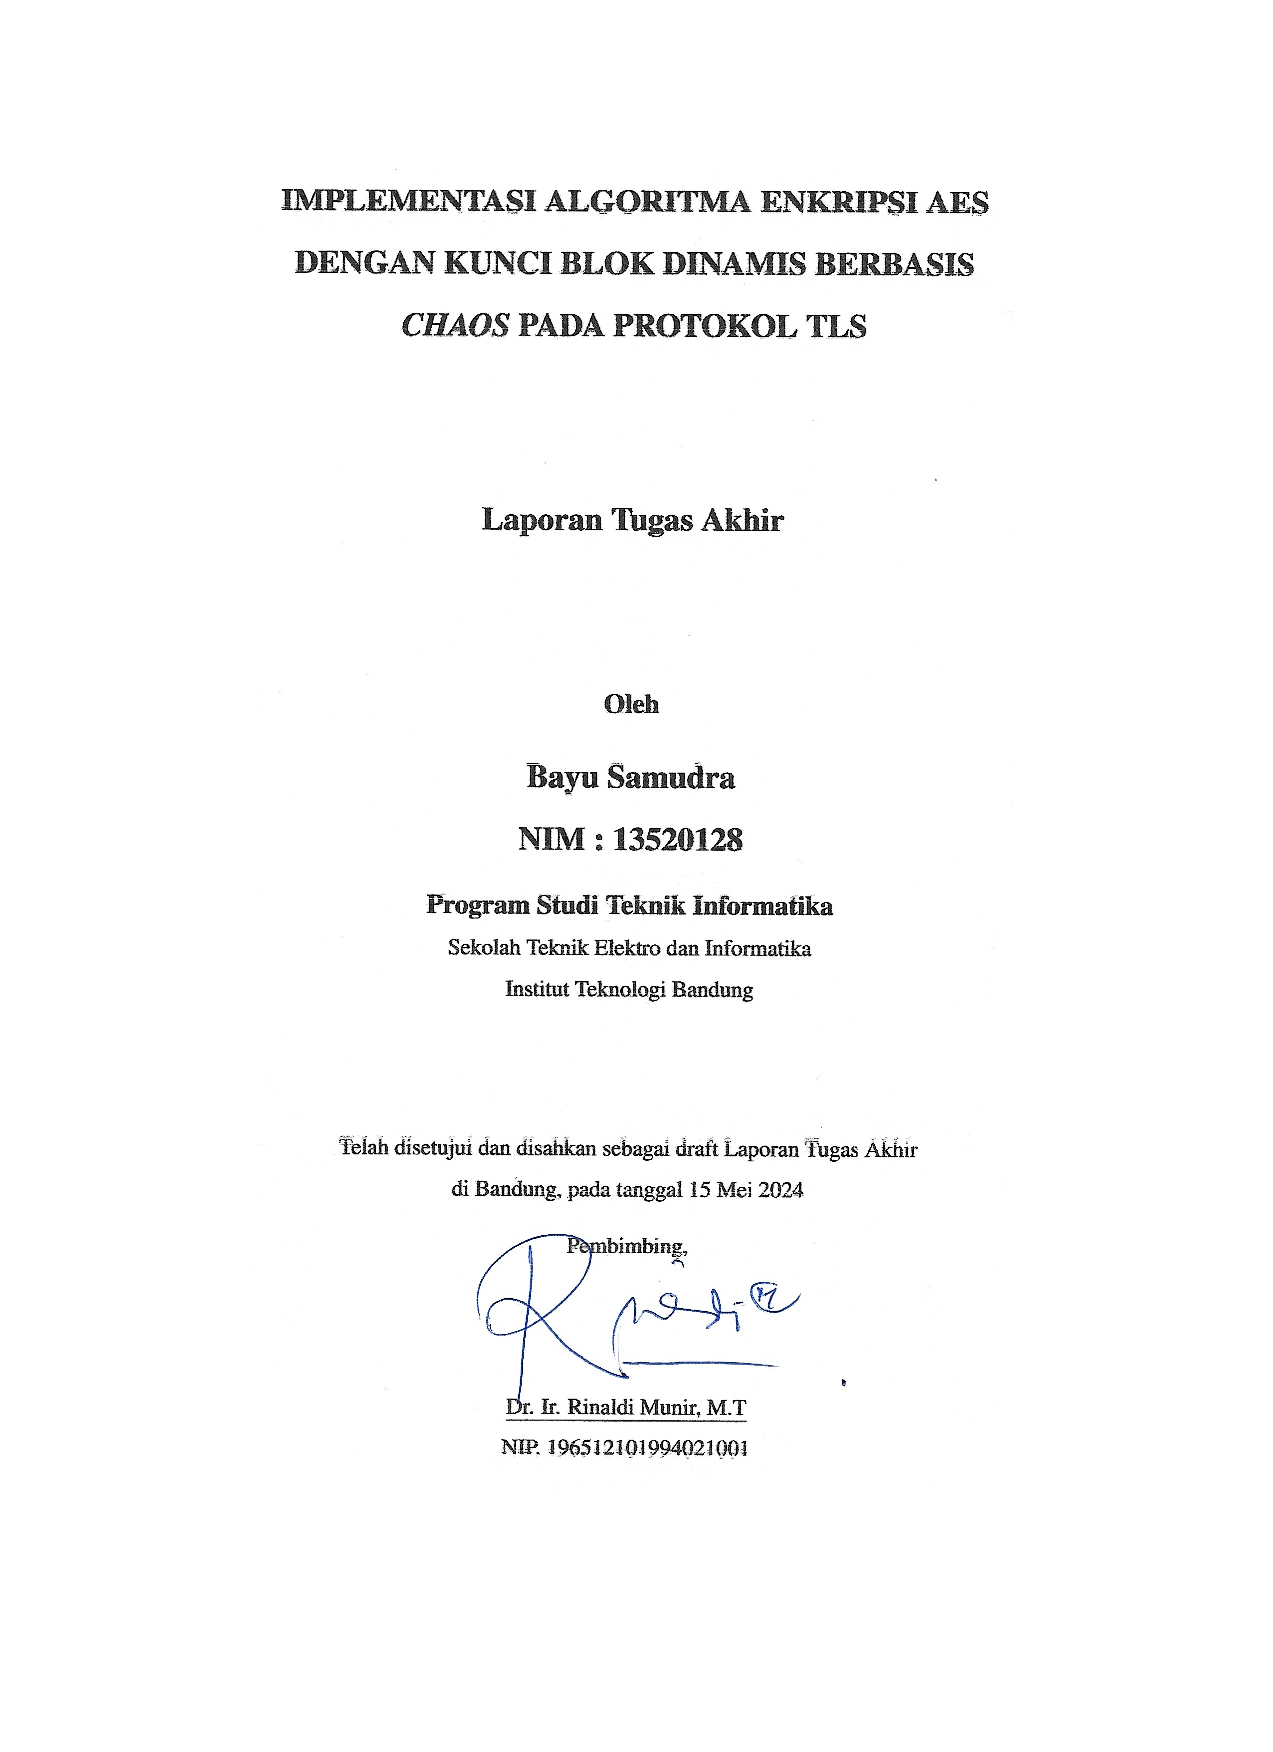
\includegraphics[scale=1]{resources/cropped_approval.pdf}
\end{center}

\clearpage

\clearpage
\pagestyle{empty}

\begin{center}
    \smallskip

    \Large \bfseries \MakeUppercase{\thetitle}
    \vfill

    \Large Laporan Tugas Akhir
    \vfill

    \large Oleh

    \Large \theauthor

    \large Program Studi Teknik Informatika \\

    \normalsize \normalfont
    Sekolah Teknik Elektro dan Informatika \\
    Institut Teknologi Bandung \\

    \vfill
    \normalsize \normalfont
    Telah disetujui dan disahkan sebagai Laporan Tugas Akhir \\
    di Bandung, pada tanggal 13 Desember 2023 \\

    \vspace{0.3cm}
    Pembimbing,

    \vspace{2cm}
    \underline{{{Dr. Ir. Rinaldi Munir, M.T}}} \\
    NIP. {{196512101994021001}}

\end{center}
\clearpage

% \clearpage
\pagestyle{empty}

\begin{center}
    \smallskip
    
    \Large \bfseries \MakeUppercase{\thetitle}
    \vfill
    
    \Large Laporan Tugas Akhir I
    \vfill
    
    \large Oleh
    
    \Large \theauthor
    
    \large Program Studi Teknik Informatika \\
    
    \normalsize \normalfont
    Sekolah Teknik Elektro dan Informatika \\
    Institut Teknologi Bandung
    
    \vfill
    \normalsize \normalfont
    Bandung, 13 Desember 2023 \\
    Mengetahui,
    
    \vspace{0.5cm}
    \setlength{\tabcolsep}{12pt}
    \begin{tabular}{c@{\hskip 0.5in}c}
        Pembimbing I,                           & Pembimbing II,                           \\
                                                &                                          \\
                                                &                                          \\
                                                &                                          \\
                                                &                                          \\
        \underline{Nama dan Gelar Pembimbing I} & \underline{Nama dan Gelar Pembimbing II} \\
        NIP. 123456789                          & NIP. 123456789                           \\
    \end{tabular}
    
\end{center}
\clearpage

% \clearpage
\pagestyle{empty}

\begin{center}
  \smallskip

  \Large \bfseries \MakeUppercase{Lembar Identitas \\ Tugas Akhir}
  \vspace{\baselineskip}

  \normalsize \normalfont
  \begin{flushleft}
    Judul Proyek TA\qquad: {{INSERT TOPIK}}
    \medskip
    
    {{ISI LEMBAR IDENTITAS...}}
    % TODO: MENUNGGU INFO UNTUK YANG NON-CAPSTONE
  \end{flushleft}
  \vfill
  Bandung, {{INSERT TANGGAL HERE}}\\
  Mengetahui,

  \vspace{0.5cm}
  Pembimbing,

  \vspace{2cm}
  \underline{{{INSERT PEMBIMBING HERE}}} \\
  NIP. {{INSERT NIP HERE}}
  \vspace{3cm}

\end{center}
\clearpage

% \chapter*{Lembar Pernyataan}

{{ISI LEMBAR PERNYATAAN DISINI...}}

{{KOTA}}, {{TANGGAL}}

\vspace{1.75cm}

{{INSERT AUTHOR HERE}}\\
NIM {{INSERT NIM HERE}}


\pagestyle{plain}

\titleformat*{\section}{\centering\bfseries\Large\MakeUpperCase}
\titlespacing*{\chapter}{0pt}{0pt}{0pc}

% \clearpage
\chapter*{ABSTRAK}
\addcontentsline{toc}{chapter}{ABSTRAK}

%taruh abstrak bahasa indonesia di sini
\begin{center}
  \center
  \begin{singlespace}
    \bfseries \MakeUppercase{\thetitle}

    \normalfont\normalsize
    Oleh:
    \bfseries \theauthor
  \end{singlespace}
\end{center}

% \vspace{1cm}

\begin{singlespace}
  Perkembangan dunia kriptografi saat ini cukup cepat. Salah satu contoh dari perkembangan kriptografi saat ini adalah \emph{cipher} dengan kunci dinamis. Terdapat beberapa penelitian yang membahas terkait hal ini, hanya saja saat ini belum ada protokol yang menerapkan \emph{cipher} ini secara nyata. Tugas akhir ini memiliki tujuan untuk mengimplementasikan algoritma enkripsi AES dengan kunci blok dinamis berbasis \emph{chaos} pada protokol TLS. Tugas akhir ini juga bertujuan untuk memilih sistem \emph{chaos} yang tepat untuk diimplementasikan pada protokol TLS. Tugas akhir ini juga menguji keamanan dari \emph{cipher} dan protokol yang dibangun. Sistem \emph{chaos} yang digunakan sebagai pembangkit kunci pada penelitian ini adalah \emph{Sine-Henon Map}. Hal ini dikarenakan sistem \emph{chaos} ini memiliki kualitas keteracakan yang baik dan menawarkan \emph{forward unpredictability}. Mode blok yang digunakan pada penelitian ini adalah \emph{counter} berbasis sistem \emph{chaos}. Hal ini diharapkan dapat meningkatkan kualitas dari hasil enkripsi. Implementasi protokol ini dilakukan pada protokol TLSv1.2. Proses implementasi dilakukan dengan menambahkan \emph{cipher suite} pada protokol TLSv1.2. Implementasi dilakukan dengan membuat sebuah pustaka. Pustaka ini dibangun dengan bahasa pemrograman Python. Pengujian  \emph{cipher} yang dilakukan adalah uji keacakan, uji ketahanan, dan uji skenario. Pengujian protokol dilakukan dengan uji skenario. Uji keacakan dilakukan dengan memanfaatkan NIST Statistical test. Uji ketahanan dilakukan dengan pengujian CCA dan MAD. Uji skenario dilakukan berdasarkan kondisi normal dan kondisi dalam serangan. Hasil pengujian menunjukan nilai acak yang dihasilkan oleh sistem \emph{chaos Sine-Henon map} memiliki kualitas yang setara dengan CSPRNG \texttt{urandom} pada sistem Linux. Hasil pengujian melalui analisis keteracakan menunjukan bahwa \emph{cipher} AES dengan kunci blok dinamis memiliki kekuatan yang setara dengan AES dengan kunci statis pada mode blok \emph{counter}. Hasil pengujian ketahanan yang dilakukan menunjukan bahwa AES dengan kunci blok dinamis memiliki kekuatan yang setara dengan AES dengan kunci statis. Hasil pengujian skenario  menunjukan bahwa protokol dan \emph{cipher} dapat bekerja dengan baik memanfaatkan \emph{cipher} kunci blok dinamis. Selain itu, protokol ini juga mampu bertahan khususnya terhadap serangan \emph{replay}, serangan MITM, dan serangan \emph{tampering}.
  
  \textbf{\textit{Kata kunci: Sine-Henon Map, TLS, AES, Sistem Chaos, Cipher Kunci Dinamis}}
\end{singlespace}
\clearpage

% % \clearpage
\chapter*{ABSTRACT}
\addcontentsline{toc}{chapter}{ABSTRACT}

\begin{center}
  \center
  \begin{singlespace}
    \bfseries \MakeUppercase{{{Implementation of AES Encryption Algorithm with Chaos-Based Dynamic Block Key on TLS Protocol}}}

    \normalfont\normalsize
    By

    \bfseries \theauthor
  \end{singlespace}
\end{center}

% \vspace{1cm}

\begin{singlespace}
  Nowadays, the Cryptography world is developing very rapidly. One development in Cryptography is dynamic keys ciphers. There are some studies about this topic, but so far, there is no protocol that implements this cipher in practice.  This final project aims to implement AES encryption with chaos-based dynamic block key on the TLS protocol. Another final project objective is selecting the appropriate chaos system that will be used as a block key generator. Also, this final project aims to test the security of the cipher and protocol that has been built. The chaos system that is used in this project is the Sine-Henon map. The reason is this chaos system has good randomness quality and offers forward unpredictability. The operation mode that is used is counter block mode. This mode is expected to improve the encryption result. The protocol implementation is done using TLSv1.2. The implementation is done by creating a python library. The security testing is done by conducting security tests in cipher and the protocol. The security tests in cipher are conducted by doing randomness test, scenario test, and robustness test. The security test in protocol is conducted by doing a scenario test. The randomness test is conducted by comparing the NIST statistical test result of the generated ciphertext by dynamic keys and static keys.  The robustness test is conducted by comparing CCA and MAD results of static and dynamic keys cipher. The scenario testing is conducted based on normal condition and attack condition. The Randomness test results show that the random value generated by the Sine-Henon map has a quality equivalent with Linux urandom. Randomness test on ciphertext shows that AES with dynamic key has a quality equivalent with static key. Scenario testing shows that the cipher can work perfectly in normal conditions and attack conditions. The protocol implementation test shows that it can work in normal conditions and attack conditions. Therefore, this protocol can work properly in normal condition and withstand from replay attack, MITM attack, and tampering attack.
  
  \textbf{\textit{Keywords: Sine-Henon Map, TLS, AES, Chaos System, Dynamic Block Cipher}}
\end{singlespace}

\clearpage

\chapter*{Kata Pengantar}
\addcontentsline{toc}{chapter}{KATA PENGANTAR}

Puji dan syukur penus panjatkan kepada Allah Subhanahu wa Ta'ala yang telah memberikan rahmat dan karunia-Nya, sehingga Penulis dapat menyelesaikan Tugas Akhir ini dengan sebaik-baiknya. Sholawat serta salam semoga selalu tercurah kepada Nabi Muhammad SAW, sebagai suri tauladan seluruh umatnya hingga akhir zaman. Laporan Tugas Akhir ini merupakan salah satu syarat kelulusan program Studi Sarjana Teknik Informatika Institut Teknologi Bandung. Laporan ini berisi terkait dengan perjalanan penulis dalam menyelesaikan Tugas Akhir yang berjudul "Implementasi Algoritma Enkripsi AES dengan Kunci Blok Dinamis Berbasis \emph{Chaos} pada Protokol TLS".

Penulis mengucapkan terima kasih kepada semua pihak yang membantu menyelesaikan Tugas Akhir ini. Khususnya kepada
\begin{enumerate}
  \item Bapak Dr. Ir. Rinaldi Munir, M.T. selaku dosen pembimbing yang telah membimbing dan mengarahkan;
  \item Bapak Yudistira Dwi Wardhana Asnar, S.T, Ph.D., Kepala Program Studi Teknik Informatika, dosen, serta rekan untuk bertukar pikiran;
  \item Orang tua yang terus memberikan dukungan serta doa;
  \item Hana Fathiyah sebagai sahabat yang selalu memberikan semangat dan dukungannya;
  \item Teman-teman Program Studi Teknik Informatika ITB angkatan 2020 yang turut memberikan dukungan.
\end{enumerate}

Dalam menulis Tugas Akhir ini, Penulis menyadari bahwa masih banyak kekurangan. Dengan demikian, Penulis mengharapkan kritik dan saran untuk kemajuan pada masa yang akan datang.

\begin{flushright}
  Cimahi, 10 Juni 2024 \\


  Bayu Samudra
\end{flushright}

\titlespacing*{\chapter}{0pt}{0pt}{1.5pc}

% Setting judul toc, lot, lof, bib
\renewcommand{\contentsname}{DAFTAR ISI}
\renewcommand{\listfigurename}{DAFTAR GAMBAR}
\renewcommand{\listtablename}{DAFTAR TABEL}
\renewcommand{\bibname}{DAFTAR REFERENSI}

\tableofcontents
\listofappendices
\listoffigures
\listoftables

% \newpage

\titleformat*{\section}{\bfseries\large}
\pagenumbering{arabic}

%----------------------------------------------------------------%
% Konfigurasi Bab
%----------------------------------------------------------------%
\setcounter{page}{1}
\renewcommand{\chaptername}{BAB}
\renewcommand{\thechapter}{\Roman{chapter}}
%----------------------------------------------------------------%

%----------------------------------------------------------------%
% Dafter Bab
% Untuk menambahkan daftar bab, buat berkas bab misalnya `chapter-6` di direktori `chapters`, dan masukkan ke sini.
%----------------------------------------------------------------%
\chapter{Pendahuluan}

\section{Latar Belakang}
Masalah keamanan informasi merupakan permasalahan yang telah muncul semenjak dahulu kala. Hal ini dikarenakan orang-orang ingin memastikan informasi yang mereka kirimkan hanyalah boleh diakses oleh orang yang memiliki wewenang untuk membukanya. Permasalahan keamanan informasi saat ini tentu saja masih menjadi yang sangat relevan. Berdasarkan data yang diunggah pada \textcite{pusiknaspolri_cybercrime_2022}, penindakan kasus kejahatan siber pada tahun tersebut meningkat dangat drastis bila dibandingkan dengan tahun sebelumnya. Hal ini memberikan tanda bahwa kejahatan siber terus berkembang. Hal ini juga diperparah dengan perkembangan teknologi dan teknik untuk melakukan peretasan semakin canggih. Oleh karena itu, diperlukan pengembangan teknik untuk melindungi data agar semakin aman.

Untuk mengamankan sebuah informasi, dapat dilakukan berbagai teknik. Salah satu teknik yang sangat penting untuk mengamankan informasi adalah kriptografi. Ilmu terkait kriptografi sudah mulai dikembangkan sejak masa dahulu kala. Hal ini dapat diamati dari kemunculan adanya \emph{Caesar Cipher}. Kemunculan dari ilmu kriptografi disebabkan oleh adanya keperluan untuk menjaga data tetap rahasia dan hanya boleh diakses oleh orang yang memiliki wewenang. Semakin berkembangnya teknologi informasi, ilmu kriptografipun turut ikut berkembang. Pada masa kini, telah terdapat beberapa  algoritma kriptografi yang dapat digunakan untuk pengiriman pesan. Menurut \textcite{munir2019}, beberapa algoritma tersebut dapat diklasifikasikan berdasarkan jumlah kunci yang terlibat dalam melakukan enkripsi dan dekripsi, yaitu kriptografi kunci simetri dan kriptografi kunci asimetris.

Menurut \textcite{halak2022}, penggunaan algoritma kunci asimetris lebih berat dibandingkan dengan penggunaan algoritma kunci simetris. Hal ini menyebabkan banyak protokol yang memanfaatkan kunci simetris dalam pertukaran pesan. Penggunaan kunci asimetris hanya digunakan untuk proses otentikasi pada saat awal dari komunikasi. Contoh dari protokol yang memanfaatkan pola seperti itu adalah \emph{Transport Layer Security} (TLS).

Menurut \textcite{munir2019}, protokol SSL/TLS membentuk kunci simetris pada saat memulai sebuah sesi komunikasi. Kunci ini disebut sebagai \emph{session key}. Hal ini menyebabkan setiap sesi dapat dipastikan memiliki kunci enkripsi yang berbeda. Akan tetapi, kunci enkripsi yang digunakan pada saat proses pertukaran data menggunakan kunci yang sama hingga sesi berakhir. Hal ini dapat menjadi celah keamanan apabila kunci enkripsi dapat diketahui oleh pihak lain.

Untuk menyelesaikan permasalahan ini, terdapat beberapa penelitian yang merancang algorithma enkripsi dinamis untuk mengenkripsi data yang dikirimkan. Pada penelitian yang dilakukan oleh \textcite{singh2019}, kedinamisan terletak pada arsitektur internal AES dalam satu \emph{round}. Penelitian ini mencoba untuk membentuk kedinamisan hasil enkripsi dengan melakukan permutasi pada S-Box, menggunakan \emph{irreducible polynomial} lain yang tersedia, serta mengganti nilai konstanta \emph{affine}. Dengan mengganti internal dalam sebuah \emph{round}, proses enkripsi tentu akan menjadi semakin kompleks. Selain itu, proses enkripsi tidak dapat dioptimasi terutama apabila CPU mendukung instruksi set yang mendukung proses menjalankan round menggunakan AES dikarenakan internal round telah berbeda.

Penelitian yang dilakukan oleh \textcite{lin2021} memanfaatkan teori \emph{chaos} untuk membangkitkan kunci yang dinamis. Selain itu, penelitian ini juga membahas terkait sinkronisasi sistem \emph{chaos} memanfaatkan \emph{sliding mode control}. Proses sinkronisasi memanfaatkan teknik tersebut memiliki sebuah kekurangan bila diimplementasikan untuk sistem enkripsi ujung ke ujung, yaitu jumlah pengiriman pesan yang perlu dilakukan selama sinkronisasi tidak konstan. Selain itu, penelitian yang dilakukan oleh \textcite{lin2021} tidak menjelaskan proses pengiriman data yang dilakukan secara dua pihak.

Dari beberapa permasalahan dan studi yang telah disebutkan, penelitian ini akan membahas pemanfaatan algoritma enkripsi simetris dinamis dalam pengiriman pesan memanfaatkan sistem \emph{chaos} pada protokol TLS. Penelitian ini akan membahas terkait mekanisme sinkronisasi \emph{state} pada protokol TLS. Selain itu, penelitian ini mencoba untuk menyelesaikan permasalahan tanpa perlu mengubah internal dari algoritma enkripsi kunci simetris.

\section{Rumusan Masalah}
Berdasarkan latar belakang yang telah dijelaskan sebelumnya, dapat disimpulkan bahwa terdapat permasalahan terkait pengiriman memanfaatkan algoritma enkripsi kunci simetris dinamis pada protokol TLS. Untuk menyelesaikan permasalahan tersebut, dibentuk beberapa rumusan masalah:
\begin{enumerate}
  \item Bagaimana cara melakukan enkripsi pesan memanfaatkan Algoritma AES kunci blok dinamis yang aman?
  \item Bagaimana cara mengimplementasikan Algoritma AES kunci blok dinamis pada protokol TLS?
\end{enumerate}

\section{Tujuan}
Penelitian ini dilakukan dengan tujuan sebagai berikut:

\begin{enumerate}
  \item Membangun sebuah protokol komunikasi berbasis TLS memanfaatkan algoritma kunci blok simetris.
  \item Menguji pengiriman pesan pada melalui protokol TLS memanfaatkan algoritma kunci blok simetris.
  \item Menguji keamanan \emph{cipher} yang telah dibuat dan implementasi dari protokol TLS.
\end{enumerate}

\section{Batasan Masalah}
Dalam penelitian ini, terdapat batasan masalah yang digunakan, yaitu sebagai berikut:
\begin{enumerate}
  \item Komunikasi dilakukan hanya oleh dua entitas.
  \item Protokol TLS yang dibangun berjalan di atas jaringan yang reliable.
  \item Proses implementasi protokol TLS hanya dilakukan hingga tahap pembuatan prototype.
\end{enumerate}

\section{Metodologi}
Metodologi yang digunakan pada penelitian ini terdapat empat tahap. Berikut ini merupakan metodologi yang digunakan pada penelitian ini:
\begin{enumerate}
  \item Analisis Masalah\\
  Penelitian pada tahap ini berfokus pada permasalahan protokol yang telah dibentuk saat ini. Pada tahap ini juga akan dijelaskan permasalahan yang mungkin muncul apabila mengimplementasikan sistem enkripsi simetris dengan kunci blok dinamis pada protokol TLS. Pada tahap ini juga akan dijelaskan terkait kebutuhan dari protokol TLS yang akan dibangun.

  \item Perancangan protokol komunikasi\\
  Setelah melakukan analisis permasalahan, perlu dilakukan perancangan solusi berupa skema protokol TLS dan sistem enkripsinya. Pada bagian ini, Penelitian mengkaji jenis mode blok yang digunakan pada protokol yang dibangun. Pada tahap ini juga, penelitian mengkaji terkait pembangkitan \emph{chaos state} berdasarkan dari kunci sesi yang telah dibentuk pada protokol TLS.

  \item Pembangunan prototype protokol komunikasi\\
  Pada tahap ini, prototype protokol komunikasi yang telah dirancang sebelumnya dibangun. Pembangunan prototype dilakukan berdasarkan perancangan desain yang telah disusun pada bagian sebelumnya. Prototype dibangun dalam bentuk program kecil yang dapat mengirimkan pesan secara bolak balik sebagai bukti bahwa protokol yang dibangun dapat berjalan.

  \item Simulasi dan Evaluasi\\
  Pada tahap ini, prototype yang telah dibuat dilakukan simulasi. Simulasi dilakukan dengan cara mengirimkan pesan berupa teks dan file binari. Hal ini dilakukan dengan menggunakan beberapa file dan teks yang berbeda. Setiap gambar yang telah diterima akan diperiksa integritasnya. Pesan terenkripsi juga akan dilakukan secara statistik dan visual. Pengujian keteracakan dilakukan dengan menggunakan NIST SP 800-22 \emph{randomness test}. Selain itu, akan dilakukan pengujian analisis entropi informasi untuk melihat keterkaitan antara satu blok dengan blok lainnya. Pengujian visual dilakukan dengan cara menampilkan gambar yang terenkripsi.
\end{enumerate}

\section{Sistematika Pembahasan}
Pembahasan pada buku laporan ini akan dibagi menjadi beberapa bab. Berikut ini merupakan sistematika penulisan pada laporan ini:

\begin{enumerate}
  \item Bab I Pendahuluan\\
  Pada bab ini, pembahasan akan berfokus pada pembahasan terkait motivasi penelitian yang tertuang pada latar belakang. Pada bab ini juga dijelaskan mengenai rumusan masalah serta tujuan dari penelitian yang dilakukan.

  \item Bab II Studi Literatur\\
  Bab ini berisi terkait teori-teori yang terkait dengan penelitian ini. Hal-hal yang dibahas pada bagian ini mencakup terkait sistem chaos, kriptografi kunci simetris AES, protokol-protokol komunikasi yang telah ada pada saat penelitian ini dilakukan, serta penelitian yang telah ada khususnya terkait dengan sistem chaos. Pada bab ini juga akan dibahas terkait protokol TLS standard.

  \item Bab III Analisis Masalah dan Rancangan Solusi\\
  Bab ini berfokus kepada analisis terkait ancaman-ancaman yang ada pada sebuah protokol komunikasi TLS. Pada bab ini juga dijelaskan terkait komposisi \emph{cipher suite} yang akan digunakan pada protokol TLS. Pada bab ini juga dijelaskan terkait rancangan protokol yang akan dibangun didasari oleh kebutuhan yang telah didefinisikan.

  \item Bab IV Implementasi Solusi dan Pengujian\\
  Pada bab ini, pembahasan akan berfokus pada implementasi dan pengujian dari protokol yang telah dijelaskan sebelumnya pada bab III. Pada bab ini akan dibahas terkait eksperimen terkait sistem \emph{chaos} yang telah dipilih. Pada bab ini juga akan dibahas terkait lingkungan protokol komunikasi yang dibangun. Selain itu, pada bab ini akan dibahas terkait hasil pengujian protokol yang telah dibangun.

  \item Bab V Kesimpulan dan Saran\\
  Bab ini berisi terkait kesimpulan dari penelitian ini. Pada bab ini juga akan diberikan saran penulis untuk penelitian yang selanjutnya.
\end{enumerate}

\chapter{Studi Literatur}

\section{Jaringan Komputer}
Menurut \textcite{forouzan2012}, jaringan komputer merupakan sebuah keterhubungan dari beberapa perangkat yang dapat melakukan komunikasi satu sama lain. Perangkat yang dapat terlibat pada jaringan komputer ini sapat berupa \emph{host} seperti komputer, laptop, dan gawai lainnya. Selain itu, perangkat pada definisi di atas dapat berupa perangkat penghubung. Beberapa contoh dari perangkat penghubung adalah \emph{router}, \emph{switch}, dan \emph{modem}.

Terdapat empat buah syarat sebuah sistem dapat dikatakan sebagai jaringan komputer menurut \textcite{pratama2015}. Syarat-syarat yang perlu dipenuhi adalah sebagai berikut:
\begin{enumerate}
  \item Dalam sebuah sistem, setidaknya terdapat dua buah perangkat yang terhubung. Perangkat tersebut dapat terhubung melalui sarana kabel (\emph{wired}) ataupun sarana nirkabel (\emph{wireless}).
  \item Pada sistem ini, terdapat pengguna yang melakukan interaksi dengan pengguna lainnya. Pengguna ini dapat berupa penyedia layanan atau seseorang yang hendak melakukan komunikasi melewati jaringan komputer.
  \item Pada sistem ini, terdapat data yang dipertukarkan di dalamnya. Jenis data yang dipertukarkan dapat berupa pesan teks ataupun pesan biner.
  \item Terdapat sebuah sumber daya yang digunakan secara bersama-sama. Sumber daya ini dapat berupa perangkat keras ataupun perangkat lunak.
\end{enumerate}

\subsection{Pemodelan Jaringan TCP/IP}
Menurut \textcite{odom2022}, pemodelan jaringan merupakan kumpulan dari berbagai dokumen yang menjelaskan sebuah fungsionalitas dalam sebuah jaringan. Dokumen-dokumen ini akan mendefinisikan hal-hal yang terjadi pada jaringan komputer saat bekerja. Beberapa dokumen bisa saja menjelaskan sebuah protokol jaringan, yaitu kumpulan aturan yang perlu dipenuhi saat sebuah perangkat melakukan komunikasi pada jaringan komputer.

Pemodelan jaringan TCP/IP merupakan pemodelan terbaru yang memperbaiki kekurangan yang ada pada pemodelan \emph{layer} OSI (\cite{forouzan2012}). Selain itu, munculnya pemodelan jaringan TCP/IP dikarenakan pemodelan OSI \emph{layer} sudah tidak relevan dalam pemodelan jaringan. Faktanya, Pemodelan jaringan OSI pada saat ini sudah tidak ada lagi (\cite{odom2022}), tetapi beberapa protokol pada pemodelan TCP/IP masih merujuk pada protokol asli yang ada pada \emph{layer} OSI.

Pemodelan jaringan TCP/IP dibagi menjadi lima lapisan. Menurut \textcite{forouzan2012}, lapisan tersebut di antaranya sebagai berikut:

\begin{enumerate}
  \item \emph{Application Layer}: Lapisan ini menjelaskan spesifikasi aplikasi agar dapat berkomunikasi dalam jaringan komputer. Lapisan ini berfungsi sebagai antar muka antara aplikasi dengan jaringan. Beberapa contoh protokol yang berada pada lapisan ini adalah HTTP, FTP, dan SSH.
  \item \emph{Transport Layer}: Lapisan ini menjelaskan cara untuk memecah paket data menjadi unit-unit data yang lebih kecil (yang disebut sebagai \emph{segment}). Selain itu, lapisan ini juga berfungsi untuk memberikan penomoran setiap unit paket data sehingga data yang didapatkan akan terurut saat diberikan kepada aplikasi. Beberapa contoh protokol yang bekerja pada tingkatan ini adalah TCP dan UDP.
  \item \emph{Network Layer}: Lapisan ini menjelaskan bagaimana sebuah paket data dalam melakukan proses \emph{routing} untuk mencapai tujuan. Pada lapisan ini, dikenal sebuah sistem pengalamatan yang disebut dengan IP (\emph{Internet Protocol}) yang terstandarisasi secara internasional.
  \item \emph{Data Link Layer}: Lapisan ini bertugas untuk mengkontrol data, mengontrol kesalahan pada data saat pengiriman, serta pengalamatan fisik. Pada lapisan ini juga, didefinisikan cara untuk mengontrol aliran paket (\emph{Flow Control}) pada sebuah jaringan.
  \item \emph{Physical Layer}: Lapisan ini bertugas untuk menjelaskan perangkat keras dari sebuah jaringan komputer. Selain itu, lapisna ini juga bertugas untuk membantu proses persinyalan dan sinkronisasi bit data.
\end{enumerate}

\subsection{Protokol TCP}
Menurut \textcite{pratama2015}, Protokol TCP merupakan protokol jaringan pada lapisan \emph{transport} yang bersifat dapat diandalkan (\emph{reliable}) dan berbasis koneksi (\emph{connection oriented}). TCP memiliki sifat keandalan dikarenakan adanya proses pemeriksaan \emph{segment} yang dikirimkan ke komputer tujuan. Hal ini terlihat adanya pesan berupa konfirmasi dari penerima. Selain itu, TCP merupakan protokol berbasis koneksi. Hal ini dikarenakan saat sebelum melakukan pengiriman data, protokol ini mengharuskan untuk membentuk koneksi jaringan komputer terlebih dahulu. 

Menurut \textcite{peterson2011}, Terdapat beberapa layanan yang disediakan oleh protokol TCP. Layanan-layanan tersebut memberikan jaminan pada aplikasi bahwa data yang diterima dapat dipastikan terurut dan tidak hilang. Beberapa layanan yang disediakan di antaranya adalah sebagai berikut.

% Semuanya dari peterson2011 %
\begin{enumerate}
  \item Keandalan (\emph{Reliability}): Pada protokol TCP, data yang dikirimkan terjamin keterurutan saat diterima oleh penerima. Selain itu, proses pengiriman pada TCP bersifat \emph{full-duplex}. Hal ini berarti proses pengiriman data dapat dilakukan dua arah secara bersama-sama. Pada protokol ini juga, terdapat mekanisme kontrol aliran data. Hal ini memungkinkan untuk pengirim atau penerima menentukan jumlah data yang dikirimkan dalam satu waktu.
  \item Berbasis koneksi (\emph{Connection Oriented}): Protokol TCP mengharuskan pembuatan koneksi pada saat sebelum pengiriman data. Proses pembentukan koneksi ini perlu untuk membangun koneksi tidak hanya pada pengirim dan penerima, tetapi juga pada seluruh perangkat jaringan yang terlibat. Selain itu, protokol TCP juga mengharuskan pemutusan koneksi saat komunikasi berakhir. 
  \item Layanan pengiriman alir: Pada TCP, aplikasi memungkinkan untuk mengirimkan \emph{byte-byte} data menuju aliran jaringan. TCP akan menentukan seberapa banyak data yang akan dikirimkan menuju penerima.
\end{enumerate}

Menurut \textcite{pratama2015}, terdapat tiga tahap koneksi yang perlu dilakukan saat mengirimkan data. Ketiga tahap tersebut adalah pembentukan koneksi, pengiriman data, serta terminasi koneksi. Ketiga tahap ini perlu dilakukan dikarenakan sifat dari protokol TCP yaitu berbasiskan koneksi.

Tahap pertama yang perlu dilakukan dalam mengirim data melalui TCP adalah pembentukan koneksi. Proses pembentukan koneksi dilakukan dengan menggunakan \emph{three way handshake}. Menurut \textcite{peterson2011}, \emph{server} membentuk koneksi pasif dengan \emph{client}. Selanjutnya, \emph{client} mengirimkan \emph{segment} ACK menuju server. Setelah server menerima \emph{segment} ACK, server akan mengirimkan \emph{segment} SYN+ACK. Setelah itu, \emph{client} mengirimkan \emph{segment} ACK menuju \emph{server}. Setelah semua proses ini terjadi, koneksi antar \emph{client} dan \emph{server} telah terjalin. Proses ini dapat digambarkan pada \ref{fig:tcp.open}. 

\begin{figure}[!h]
  \centering
  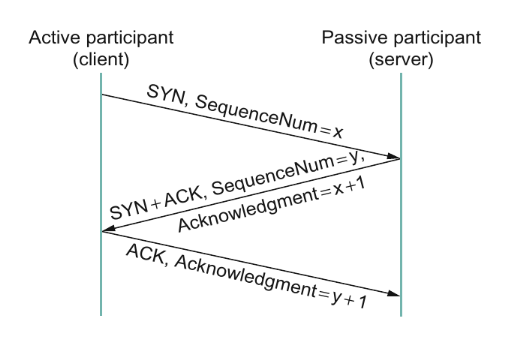
\includegraphics[width=280px]{chapters/res/chapter-2/img/tcp.open.png}
  \caption{Proses Pembukaan Koneksi TCP} \label{fig:tcp.open}
  Sumber: \textcite{peterson2011}
\end{figure}

Saat koneksi telah terjalin, pengiriman data sudah dapat dilakukan. Proses transfer data dilakukan dengan mengirimkan \emph{segment} data menuju penerima. Saat menerima data, penerima harus mengirimkan \emph{segment} ACK menuju pengirim. Apabila terjadi kegagalan transmisi, setiap \emph{segment} yang hilang harus ditransmisikan ulang.

Menurut \textcite{peterson2011}, setiap \emph{segment} yang dikirimkan diharapkan selalu penuh. Hal ini mencegah terjadi permasalahan \emph{silly window syndrome}. Oleh karena itu, pengiriman dapat diatur oleh algoritma nagle. Terdapat sebuah parameter untuk menentukan besar maksimum data yang dikirimkan yaitu nilai \emph{maximum segment size} (MSS).

Pada saat pengiriman data, terdapat juga sebuah nilai $Timeout$ yang menentukan apakah proses pengiriman \emph{segment} perlu diulang. Nilai ini dapat diturunkan melalui nilai estimasi \emph{round time trip} (RTT) dari sebuah data. Saat mengirimkan data, pengirim perlu menunggu ACK hingga batas $timeout$. Apabila telah terjadi timeout, pengirim perlu mengirimkan ulang data mereka menuju penerima. Semua proses pada tahap pengiriman ini perlu dilakukan hingga semua data berhasil dikirimkan.

Pada fase terakhir, koneksi antara \emph{client} dan \emph{server} perlu ditutup. Hal ini perlu dilakukan dengan \emph{client} melakukan proses \emph{active close}. Pada tahap \emph{active close}, \emph{client} mengirimkan pesan FIN. Setelah itu, \emph{server} mengirimkan pesan FIN+ACK. Setelah menerima pesan dari \emph{server}, \emph{client} perlu mengirimkan ACK. Setelah itu, koneksi antara \emph{server} dan \emph{client} telah tertutup.

\section{Kriptografi}
Menurut \textcite{schneier1996}, Kriptografi merupakan ilmu pengetahuan dan seni yang berujuan untuk menjaga sebuah pesan tetap aman. Menurut \textcite{anderson2008}, Kriptografi dianggap sebagai pintu para pengembang keamanan untuk bertemu dengan ilmu matematika. Hal ini dapat terlihat bahwa banyak sekali algoritma kriptografi yang terkait dengan konsep matematika. Kriptografi dianggap juga sebagai seni. Menurut \textcite{munir2019}, hal ini dikarenakan dari pandangan sejarah berkembangnya kriptografi. Kriptografi ini terbentuk dikarenakan adanya keinginan untuk merahasiakan sebuah pesan. Tentu saja, setiap orang memiliki ciri khas serta caranya tersendiri untuk menyandikan sebuah pesan. Oleh karena itu, kriptografi dapat dianggap sebagai seni untuk merahasiakan sebuah pesan. 

Kriptografi pada dasarnya memiliki beberapa layanan dasar yang dapat digunakan dalam dunia keamanan. Menurut \textcite{schneier1996}, beberapa layanan yang terdapat pada kriptografi adalah sebagai berikut:
\begin{enumerate}
  \item Kerahasiaan (\emph{confidentiality}) merupakan sebuah layanan yang diberikan oleh kriptografi untuk menjaga pesan agar pesan hanya dapat dimengerti oleh pihak yang memiliki otoritas. 
  \item Integritas (\emph{integrity}) merupakan layanan yang menjamin bahwa pesan yang diterima merupakan pesan yang belum pernah dilakukan modifikasi sebelumnya. Layanan ini menjamin data yang diterima sama dengan data tersebut saat pertama kali dikirim.
  \item Otentikasi (\emph{authentication}) merupakan layanan yang menjamin bahwa pesan yang diterima merupakan pesan yang dikirim oleh pengirim sesungguhnya. Hal ini terkait dengan klaim bahwa pesan yang dikirimkan tentu saja dapat dilakukan dekripsi dengan kunci yang telah disepakati.
  \item Anti penyangkalan (\emph{non-repudiation}) merupakan layanan yang menjamin bahwa pengirim tentu saja tidak akan dapat menyangkal pesan yang telah dia kirimkan.
\end{enumerate} 

Kriptografi modern, menurut \textcite{munir2019}, merupakan kriptografi yang bekerja pada komputer digital. Pesan tidak hanya terbatas pada tulisan dan alfabet, namun pesan juga dapat berupa berbentuk apapun selama dapat diubah menjadi bentuk biner. Dalam Kriptografi modern, terdapat sebuah konsep yang disebut dengan kriptografi kunci publik, konsep fungsi \emph{hash}, serta tanda tangan digital. Hal ini merupakan konsep baru yang dapat digunakan untuk menjamin integritas serta anti penyangkalan dari pengirim pesan.

Menurut \textcite{schneier1996}, keamanan kriptografi modern tidak hanya cukup apabila merahasiakan algoritma penguncian. Hal ini dikarenakan apabila sebuah algoritma penguncian dapat dipecahkan, algoritma tersebut perlu diganti dengan yang baru. Dalam kriptografi modern, kerahasiaan yang perlu dijaga terletak pada kunci. Setiap operasi enkripsi serta dekripsi tentu saja akan melibatkan kunci ini. 

Sebuah algoritma kriptografi tentu membutuhkan kunci untuk melakukan proses enkripsi dan dekripsi. Menurut \textcite{schneier1996}, algoritma kriptografi dapat dibagi menjadi dua, yaitu Kriptografi kunci simetrik dan kriptografi publik. Perbedaan dari kedua algoritma tersebut terletak pada kunci yang digunakan untuk melakukan enkripsi serta dekripsi pesan. 

Menurut \textcite{munir2019}, algoritma kunci simetri menggunakan kunci yang sama saat melakukan proses enkripsi serta dekripsi pesan. Asumsi yang diterapkan pada penggunaan algoritma ini adalah pengirim serta penerima sudah melakukan proses pembagian kunci. Skema proses enkripsi digambarkan pada gambar \ref{fig:crypto.symetric}.

\begin{figure}[!h]
  \centering
  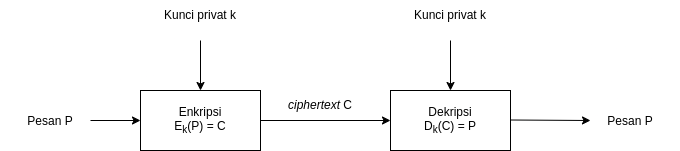
\includegraphics[width=\textwidth]{chapters/res/chapter-2/img/crypto.symetric.png}
  \caption{Visualisasi Proses Enkripsi Kriptografi Kunci Simetri} \label{fig:crypto.symetric}
  Sumber: \textcite{munir2019}
\end{figure}

Menurut \textcite{munir2019}, algoritma kriptografi kunci simetris ini dibagi lagi menjadi dua buah jenis, yaitu \emph{cipher} blok dan \emph{cipher} alir. Perbedaan antara kedua jenis \emph{cipher} tersebut terletak pada cara pengenkripsian sebuah pesan. Pada \emph{cipher} alir, proses enkripsi dilakukan dengan cara mengenkripsikan pesan per bit per bit. Proses penenkripsian juga tidak menutup kemungkinan dilakukan \emph{byte} per \emph{byte}. Contoh algoritma yang termasuk dalam \emph{cipher} alir adalah RC4 dan A5.

Menurut \textcite{munir2019}, Algoritma \emph{cipher} blok merupakan algoritma kunci simetris yang memproses pesan berdasarkan blok-blok bit atau \emph{byte}. Enkripsi dilakukan pada blok tersebut setiap kali. Terdapat beberapa operasi yang ada pada \emph{cipher} blok, di antaranya adalah ECB, CBC, CFB, dan OFB. Setiap operasi ini menentukan cara setiap blok pesan \emph{plaintext} atau \emph{ciphertext} dilakukan proses kriptografi.


\begin{figure}[!h]
  \centering
  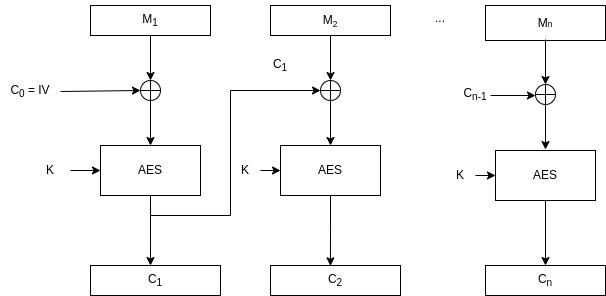
\includegraphics[width=\textwidth]{chapters/res/chapter-2/img/cbc.encrypt.png}
  \caption{Visualisasi Enkripsi Mode Blok CBC} 
  \label{fig:crypto.cbc.encrypt}
  Sumber: \textcite{munir2019}
\end{figure}


\begin{figure}[!h]
  \centering
  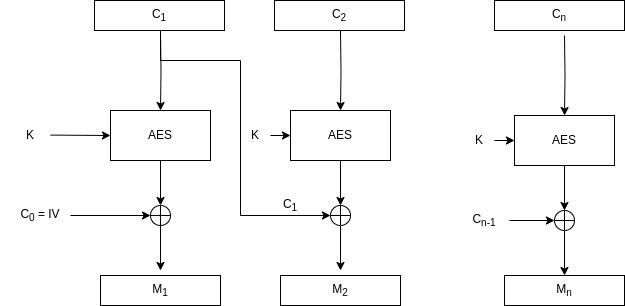
\includegraphics[width=\textwidth]{chapters/res/chapter-2/img/cbc.decrypt.png}
  \caption{Visualisasi Dekripsi Mode Blok CBC} 
  \label{fig:crypto.cbc.decrypt}
  Sumber: \textcite{munir2019}
\end{figure}

Salah satu bentuk mode blok yang sering digunakan dalam melakukan enkripsi adalah CBC. Menurut \textcite{munir2019}, mode enkripsi CBC menerapkan sistem enkripsi dengan cara memanfaatkan umpan balik dari hasil enkripsi blok sebelumnya. Nilai blok yang akan dienkripsi pertama-tama akan dilakukan XOR terlebih dahulu dengan umpan balik tersebut. Setelah itu, hasil XOR akan dienkripsi dengan kunci $K$. Nilai umpan balik awal disebut dengan $IV$. Nilai $IV$ tidak perlu dirahasiakan, tetapi perlu dibuat secara acak saat hendak melakukan proses enkripsi. Ilustrasi proses enkripsi menggunakan blok ini diilustrasikan pada gambar \ref{fig:crypto.cbc.encrypt}, sedangkan ilustrasi proses dekripsi digambarkan pada gambar \ref{fig:crypto.cbc.decrypt}. Secara matematis, proses ini ditunjukan pada persamaan \ref{eq:crypto.cbc.enc}.

\begin{equation}
  \label{eq:crypto.cbc.enc}
  \begin{array}{l}   
    Ct_i = E_K(P_i \oplus C_{i-1}) \\
    Pt_i = D_K(C_i) \oplus C_{i-1} \\
    C_0 = IV
  \end{array}
\end{equation}

Menurut \textcite{munir2019}, terdapat keuntungan saat menggunakan mode blok CBC dalam melakukan enkripsi. Keuntungan utamanya adalah hasil enkripsi akan memberikan hasil cipherteks yang berbeda untuk plainteks yang sama. Hal ini disebabkan adanya persebaran informasi antar tiap blok sehingga hasil enkripsi kedua blok tersebut dapat berbeda. Akan tetapi, kelemahan utama mode blok ini adalah perubahan satu bit pada cipherteks dapat membalikan satu bit pada blok setelahnya. Hal ini dapat digunakan pihak lawan untuk melakukan \emph{bit-flip attack} dengan memanfaatkan sifat ini. 

Menurut \textcite{munir2019}, algoritma kunci publik (atau bisa disebut algoritma kunci nirsimetris) merupakan algoritma enkripsi yang menggunakan kunci yang berbeda pada saat melakukan proses enkripsi dan juga proses dekripsi. Pada saat melakukan komunikasi menggunakan algoritma ini, pihak yang terlibat harus memiliki satu buah kunci, yaitu kunci publik dan kunci privat. Pengirim pesan akan menggunakan kunci publik untuk mengunci pesan. Akan tetapi, penerima menggunakan kunci privat miliknya untuk membuka pesan. Dengan menggunakan algoritma ini, hanya penerima pesan yang dapat membuka pesan. Ilustrasi terkait enkripsi memanfaatkan algoritma ini terdapat pada gambar \ref{fig:crypto.asymetric}. Beberapa contoh algoritma enkripsi kunci publik adalah RSA, \emph{Elgamal}, dan DSA.

\begin{figure}[!h]
  \centering
  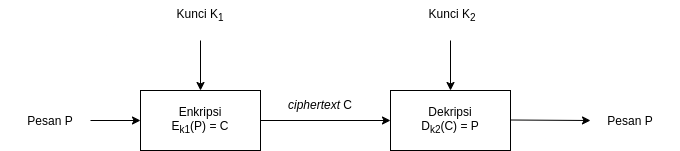
\includegraphics[width=\textwidth]{chapters/res/chapter-2/img/crypto.asymetric.png}
  \caption{Visualisasi Proses Enkripsi Kriptografi Kunci Publik} 
  \label{fig:crypto.asymetric}
  Sumber: \textcite{munir2019}
\end{figure}

Menurut \textcite{munir2019}, kriptografi kunci publik adadapat memberikan dua keuntungan. Keuntungan pertama adalah tidak adanya kebutuhan dalam mendistribusikan kunci rahasia. Kunci publik dapat dikirimkan melalui saluran yang tidak aman. Selain itu, keuntungan lain dari penggunaan kunci publik ini adalah jumlah pembuatan kunci dapat dikurangi. Pada saat menggunakan kriptografi kunci simetri, jumlah kunci yang harus dibuat adalah sebanyak jumlah pihak yang ingin berkomunikasi. Pada saat menggunakan algoritma asimetris, kunci yang perlu dibuat hanyalah sebanyak dua buah kunci, sehingga jumlah kunci menjadi lebih sedikit.

\section{Enkripsi Dinamis}
Enkripsi dinamis pertama kali dikenalkan oleh \textcite{knudsen2015}. Menurut \textcite{knudsen2015}, Enkripsi dinamis merupakan sebuah pendekatan kriptografi yang menyebabkan penerima pesan tidak perlu mengetahui detail proses enkripsi selain nilai dari \emph{secret key} dalam melakukan proses dekripsi. Pengirim pesan dapat menentukan algoritma enkripsi yang akan digunakan. Akan tetapi, penerima pesan tidak perlu mengetahui proses enkripsi yang dilakukan. Hal ini tentu mengharuskan bahwa penerima pesan dapat melakukan porses dekripsi dengan baik walaupun proses enkripsi tidak diketahui. 

Terdapat beberapa pendekatan yang ditawarkan oleh \textcite{knudsen2015}, salah satunya adalah dengan cara mengirimkan algoritma dekripsi $D$ ke penerima pesan. Pemilihan algoritma enkripsi dilakukan secara acak oleh pengirim. Pengiriman ini dilakukan dengan cara mengenkripsi algoritma $D$ dengan sistem enkripsi yang telah disepakati oleh kedua pihak. Penerima akan menjalankan algoritma dekripsi yang diterima untuk mendekripsi pesan. Berdasarkan \textcite{knudsen2015}, kelemahan dari pendekatan ini adalah transmisi kode \emph{executable}. Kode ini pun perlu dijalankan di penerima sehingga dapat membahayakan pengguna apabila kode yang dibuat merupakan kode yang berbahaya. Untuk mengatasi hal ini, diberikan beberapa solusi diantaranya adalah dengan memberikan pengecekan integritas dan otentikasi. Selain itu, perlu dilakukan juga pembatasan lingkungan eksekusi untuk melakukan proses dekripsi.

Menurut \textcite{knudsen2015}, terdapat varian lain dalam melakukan enkripsi dinamis, yaitu dengan menggunakan \emph{cipher} RAES. Pada \emph{cipher} RAES, proses enkripsi dilakukan sebagaimana AES-128 dilakukan. Akan tetapi, S-box yang digunakan berbeda. Terdapat dua buah kunci yang digunakan dalam melakukan enkripsi, yaitu kunci untuk digunakan pada AES-128 dan kunci untuk membangkitkan S-box. Menurut \textcite{knudsen2015}, keamanan menggunakan metode ini setidaknya sama kuatnya dengan menggunakan S-box.

\section{Pertukaran Kunci \emph{Diffie–Hellman}}
Algoritma pertukaran kunci \emph{Diffie–Hellman} merupakan algoritma yang digunakan untuk berbagi kunci sesi antara dua pihak atau lebih. Menurut \textcite{munir2019}, algoritma pertukaran kunci \emph{Diffie–Hellman} merupakan solusi dari permasalahan kriptografi kunci simetri, yaitu pengiriman kunci pada komunikasi jaringan yang tidak aman. Secara garis besar, setiap pihak yang akan melakukan pertukaran kunci menggunakan \emph{Diffie–Hellman}, akan mengirimkan parameter publiknya kepada setiap pihak. Penerima parameter publik akan membangkitkan kunci sesi berdasarkan parameter publik yang diterima dan parameter privat yang dimiliki olehnya. Ilustrasi pertukaran kunci ini digambarkan pada \ref{fig:crypto.dh}.

\begin{figure}[!h]
  \centering
  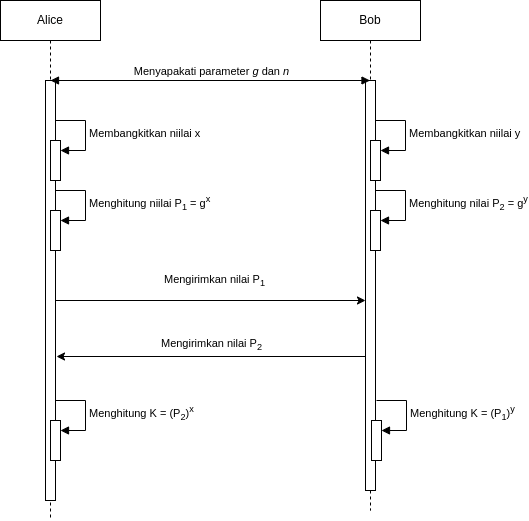
\includegraphics[width=\textwidth]{chapters/res/chapter-2/img/crypto.dh.png}
  \caption{Visualisasi Pertukaran Kunci \emph{Diffie-Hellman}} \label{fig:crypto.dh}
  Sumber: \textcite{munir2019}
\end{figure}

Pada ilustrasi yang ditunjukan \ref{fig:crypto.dh}, setiap pihak akan mendapatkan nilai $K$ yang sama. Nilai $K$ ini akan digunakan sebagai kunci sesi pada saat melakukan enkripsi menggunakan algoritma enkripsi kunci simetris.

Kekuatan dari pertukaran kunci \emph{Diffie–Hellman} menurut \textcite{munir2019} terletak pada sulitnya melakukan operasi logaritma diskrit. Nilai $x$ dan $y$ yang ditunjukan pada ilustrasi \ref{fig:crypto.dh} hanya dapat diekstrasi bila melakukan operasi logaritma diskrit dengan basis $g$. Menurut \textcite{staling2011}, Algoritma paling baik untuk mencari nilai logaritma diskrit saat ini berada pada kompleksitas $O(e^{(\ln{p})^{1/3} \cdot (\ln{(\ln{p})})^{2/3}})$ sehingga masih belum cukup mangkus untuk menyelesaikan persoalan ini untuk nilai $p$ yang besar.

\section{\emph{Advanced Encryption Standard (AES)}}
Menurut \textcite{staling2011}, Advanced Encryption Standard (AES) merupakan sebuah salah satu algoritma cipher blok yang dibuat dengan tujuan untuk menggantikan algoritma DES. Berdasarkan panjang kunci, algoritma AES dapat dibagi menjadi tiga, yaitu AES-128, AES-192, dan AES-256. Cipher AES akan melakukan enkripsi dan dekripsi dalam sejumlah \emph{round}. Jumlah \emph{round} yang akan dilakukan bergantung terhadap panjang kunci yang digunakan. Tabel \ref{tab:aes-round} menunjukan jumlah round yang digunakan pada spesifikasi algoritma AES.

\begin{longtable}{|c|c|}
  \caption{\label{tab:aes-round} Tabel Panjang Kunci dan Jumlah Round pada Algoritma AES} \\
  \hline
  Panjang Kunci & Jumlah Round \\ \hline
  128 bit       & 10           \\ \hline
  192 bit       & 12           \\ \hline
  256 bit       & 32           \\ \hline
\end{longtable}

Menurut \textcite{staling2011}, AES memiliki empat tahap yang digunakan dalam melakukan proses enkripsi. Tahap-tahap yang dilakukan dalam algoritma \emph{Rijndael} diantaranya adalah sebagai berikut:

\begin{enumerate}
  \item Tahap \emph{AddRoundKey}\\Menurut \textcite{munir2019}, Nilai \emph{state} akan dilakukan operasi XOR terhadap \emph{round key} pada tahap ini. Nilai \emph{round key} akan dibangkitkan melalui aloritma ekspansi kunci sehingga setiap \emph{round} akan memiliki kunci yang berbeda-beda.  
  \item Tahap Transformasi \emph{ShiftRow}\\Menurut \textcite{munir2019}, Nilai \emph{state} akan dilakukan pergeseran baris matriks secara \emph{wrapping}. Operasi ini bertujuan untuk mengubah urutan dalam plainteks. Jumlah pergeseran yang dilakukan ditentukan dengan posisi elemen baris pada matriks \emph{state}.
  \item Tahap \emph{MixColumns}\\Menurut \textcite{munir2019}, tahap ini merupakan pengacakan yang dilakukan pada nilai \emph{state}. Pada tahap ini, nilai \emph{state} akan dikalikan dengan matriks tertentu. Operasi perkalian yang digunakan merupakan perkalian pada $GF(2^8)$, sedangkan operasi penjumlahan yang digunakan merupakan XOR.
  \item Tahap \emph{Subtitute Bytes}\\Menurut \textcite{munir2019}, tahap ini merupakan tahap substitusi berdasarkan sebuah tabel yang bernama S-Box. Pada tahap ini, nilai pada \emph{state} akan dipetakan nilainya berdasarkan S-box yang digunakan. AES hanya memiliki sebuah table S-box yang digunakan pada setiap putaran serta pembangkitan kunci.
\end{enumerate}

Secara garis besar, proses enkripsi melalui algoritma \emph{Rijndael} ini ditunjukan pada gambar \ref{fig:crypto.aes}.


\begin{figure}[!h]
  \centering
  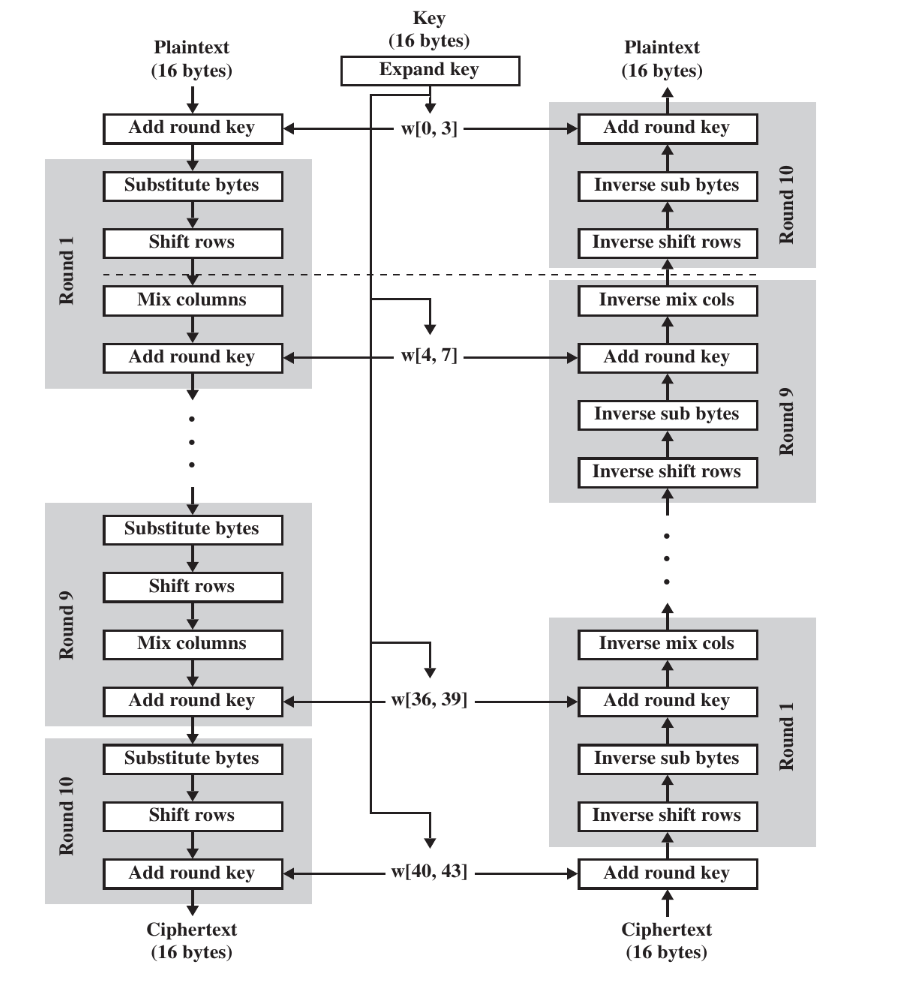
\includegraphics[width=\textwidth]{chapters/res/chapter-2/img/crypto.aes.png}
  \caption{Visualisasi Proses Enkripsi dan Dekripsi pada AES} \label{fig:crypto.aes}
  Sumber: \textcite{staling2011}\text

\end{figure}

\section{CSRPNG Berbasis \emph{Chaos}}
Menurut \textcite{munir2019}, Sistem chaos merupakan sistem matemtis yang dapat menghasilkan nilai dengan tidak teratur. Sistem chaos sangat peka terhadap perubahan kecil. Hal ini dikarenakan sistem chaos memiliki fenomena efek kupu-kupu.

Berdasarkan \textcite{boris2003}, terdapat tiga buah syarat sebuah sistem matematis dapat sebagai sistem chaos. Syarat tersebut diantaranya adalah sebagai berikut:
\begin{enumerate}
  \item Sistem tersebut haruslah sensitif terhadap nilai awal.
  \item Sistem tersebut harus memenuhi sifat \emph{topological transitive}. Hal ini berarti setiap nilai pada sistem chaos haruslah dapat dicapai dengan melakukan operasi sebuah fungsi secara berulang (\textcite{boris2003}).
  \item Sistem tersebut juga haruslah memiliki orbit periode yang padat.
\end{enumerate}

Menurut \textcite{munir2019}, Salah satu sifat yang dimiliki oleh sistem \emph{chaos} adalah ia bersifat deterministik. Selain itu, sistem chaos memiliki ketidakteraturan yang tinggi dalam menghasilkan nilai. SIfat yang paling penting adalah peka terhadap nilai awal. Semua sifat ini dapat memberikan sifat difusi pada algoritma kriptografi dikarenakan sistem chaos ini dapat menghilangkan hubungan statistik pada ciperteks.

Terdapat berbagai contoh dari sistem \emph{chaos} yang telah didefinisikan pada berbagai sumber. Menurut \textcite{munir2019}, Salah satu contoh fungsi \emph{chaos} yang sederhana adalah sistem \emph{chaos} berbasiskan persamaan logistik. Persamaan logistik didefinisikan pada persamaan \ref{eq:chaos.logistic}.

\begin{equation}
  \label{eq:chaos.logistic}
  X_{n+1} = r X_n (1 - X_n)
\end{equation}

Pada persamaan \ref{eq:chaos.logistic}, nilai $r$ menyatakan laju pertumbuhan. Nilai $r$ menentukan kemunculan sifat chaos dari persamaan logistik. Berdasarkan \textcite{munir2019}, fungsi logistik sepenuhnya memiliki sifat chaos saat $r = 4$. Hal ini dikarenakan proses \emph{bifurcation} sangat cepat terjadi. Fenomena \emph{bifurcation} merupakan fenomena saat fungsi terpecah menjadi dua sehingga fungsi akan terus berosilasi pada dua populasi nilai tersebut. Saat proses  \emph{bifurcation} terjadi sangat cepat, sifat dari sistem akan sulit sekali diprediksi. Oleh karena itu, hal ini sangat cocok bila dimanfaatkan sebagai CSRPNG berbasis sistem \emph{chaos}.

Selain sistem \emph{chaos} berbasiskan persamaan logistik, terdapat sistem chaos memanfaatkan peta hénon. Berdasarkan \textcite{henon1976}, persamaan peta hénon didefinisikan sebagaimana persamaan \ref{eq:chaos.henon}.

\begin{equation}
  \label{eq:chaos.henon}
  \begin{array}{l}   
  X_{n+1} = Y_{n} + 1 - aX_{n}^2 \\
  Y_{n+1} = bX_{n} 
  \end{array}
\end{equation}

Menurut \textcite{aybar2013}, untuk nilai $b = 0.3$ dihasilkan peta \emph{bifurcation} yang ditunjukan pada gambar \ref{fig:henon.bifurcation}. gambar \ref{fig:henon.bifurcation} memperlihatkan bahwa saat nilai $a$ mendekati $1.2$, sifat \emph{chaos} terjadi. Hal ini terjadi dikarenakan proses \emph{bifurcation} terjadi sangat cepat sehingga muncul sifat \emph{chaos} pada sistem tersebut.

\begin{figure}[!h]
  \centering
  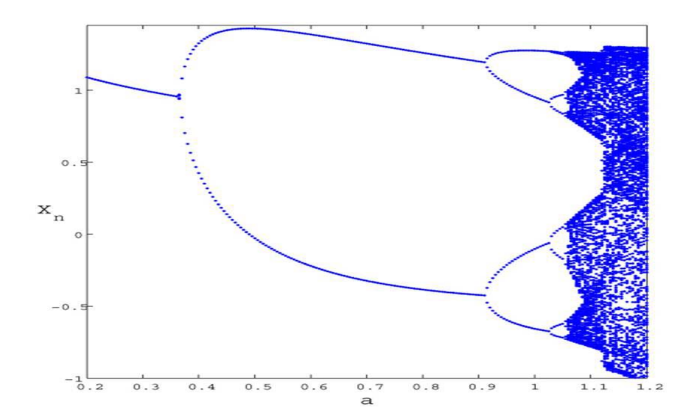
\includegraphics[width=\textwidth]{chapters/res/chapter-2/img/henon.bifurcation.png}
  \caption{Diagram \emph{bifurcation} pada peta hénon dengan nilai $0.2 \ge a \ge 1.2$ dan $b = 0.3$} \label{fig:henon.bifurcation}
  Sumber: \textcite{aybar2013}
\end{figure}

Menurut \textcite{munir2019}, untuk membangkitkan nilai bilangan bulat, sistem \emph{chaos} haruslah dilakukan konversi menuju bilangan bulat. Salah satu fungsi yang dapat digunakan dalam melakukan konversi ini dinyatakan pada persamaan \ref{eq:chaos.linearization}.

\begin{equation}
  \label{eq:chaos.linearization}
  T(x, n) = \lfloor x \cdot 10^n \rfloor
\end{equation}

\section{Message Authentication Code (MAC)}
Menurut \textcite{munir2019}, Fungsi hash satu arah merupakan fungsi yang dapat menghasilkan sebuah \emph{message digest} yang tidak dapat dikembalikan menjadi pesan sesungguhnya. Dua pesan berbeda dapat menghasilkan nilai hash yang berbeda. Beberapa contoh fungsi hash adalah MD5 dan SHA-256.

Menurut \textcite{munir2019}, MAC merupakan perbaikan dari permasalahan yang muncul apabila menggunakan pengecekan integritas data memanfaatkan nilai hash. Dalam menjaga integritas sebuah data dengan menggunakan nilai hash saja, dapat menimbulkan kerentanan apabila data dan nilai hash diubah. MAC merupakan sebuah fungsi \emph{hash} satu arah yang menggunakan kunci rahasia dalam pembangkitannya.

\begin{figure}[!h]
  \centering
  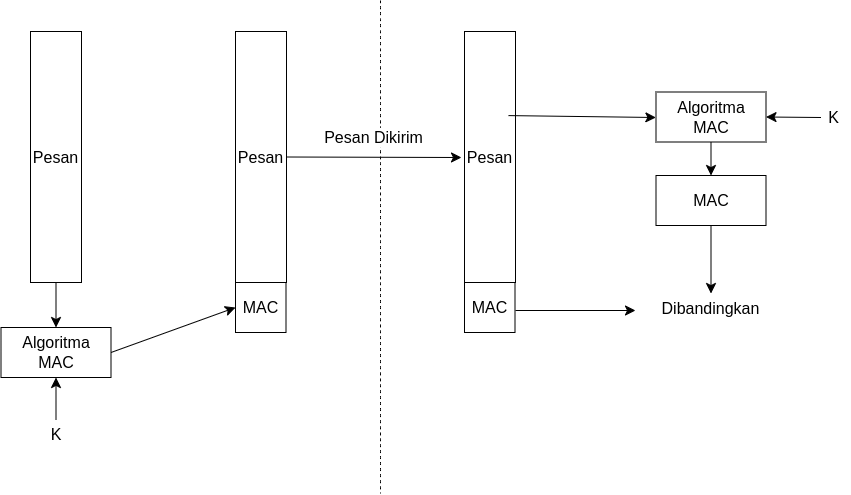
\includegraphics[width=350px]{chapters/res/chapter-2/img/mac.png}
  \caption{Ilustrasi proses pengiriman dan verifikasi pesan dengan MAC} \label{fig:mac}
  Sumber: \textcite{munir2019}
\end{figure}

Menurut \textcite{munir2019}, MAC dapat digunakan sebagai otentikasi pesan tanpa perlu melakukan enkripsi pada pesan tersebut. Hal ini dapat dilakukan dengan cara melekatkan nilai MAC pada pesan yang dikirimkan. Proses tersebut digambarkan pada gambar \ref{fig:mac}. Proses verifikasi pesan dilakukan dengan membandingkan nilai MAC dari pesan yang dihitung ulang berdasarkan pesan yang diterima dengan nilai MAC yang dikirimkan. Apabila pesan tidak diubah, kedua nilai ini menghasilkan nilai yang sama. Keuntungan menggunakan MAC ini adalah adanya nilai $K$ sehingga nilai hash yang dilekatkan pada pesan tidak secara mudah dapat diganti.

\section{Penelitian Terkait}

Penelitian terkait enkripsi dinamis telah dilakukan oleh beberapa pihak. Berikut ini adalah beberapa penelitian yang berkaitan dengan enkripsi dinamis. 

\subsection{Sinkronisasi Kunci Dinamis berbasis Chaos den Aplikasinya pada Pengenkripsian gambar dengan Algoritma AES yang diimprovisasi}

Menurut \textcite{lin2021}, kebutuhan keamanan data untuk berkomunikasi terus meningkat. Hal ini dikarenakan perkembangan sistem multimedia saat ini tentu terus berkembang. Salah satu variasi pengembangan algoritma enkripsi dan dekripsi yang berkembang saat ini menerapkan sinyal \emph{chaos}. 

Untuk memanfaatkan sistem \emph{chaos}, diperlukan sebuah parameter berupa nilai inisialisasi dari sistem chaos. Nilai ini perlu dipertukarkan melalui jaringan yang tidak aman, sehingga menambah peluang nilai tersebut dapat di-\emph{crack}. Terdapat beberapa pendekatan biasa dilakukan untuk mencapai sinkronisasi, yaitu menggunakan \emph{backstepping design}, \emph{fuzzy control}, dan \emph{sliding mode control}. Dari ketiga metode tersebut, mode yang sering digunakan adalah mode \emph{sliding mode control}. Penelitian yang dilakukan oleh (\cite{lin2021}) salah satunya akan berbicara terkait sinkronisasi sistem \emph{chaos} ini.

Penelitian ini juga termotivasi dengan adanya beberapa serangan yang biasa dilakukan oleh \emph{cracker} untuk memecahkan pesan \emph{ciphertext} memanfaatkan algoritma AES. Salah satu metode untuk melakukan serangan adalah memanfaatkan nilai \emph{cache}. Hal ini dapat terjadi dikarenakan pada saat ini, proses enkripsi menggunakan kunci simetri masih menggunakan kunci yang statis. Apabila kunci ini berhasil untuk dicuri, semua \emph{ciphertext} yang ada dapat dengan mudah untuk dilakukan dekripsi. Selain itu, perkembangan komputer kuantum juga menjadi tantangan tersendiri bagi AES. Komputer kuantum dapat memecahkan enkripsi AES dengan waktu yang cukup cepat. Oleh karena itu, penelitian ini juga terkait dengan modifikasi algoritma AES berbasis \emph{chaos} memanfaatkan kunci dinamis yang tersinkronisasi. Pengujian hasil dari algoritma AES berbasis \emph{chaos} ini dilakukan dengan cara melakukan enkripsi pada sebuah gambar. Analisis yang dilakukan diantaranya adalah analisis statis, histogram, entropi informasi, dan korelasi untuk menguji keamanan dan efisiensi dari algoritma yang telah dibentuk.

Pada penelitian \textcite{lin2021}, digunakan sistem \emph{chaos} berbasis Henon maps. Nilai \emph{chaos} ini dibagi menjadi dua buah bagian, yaitu \emph{master} dan \emph{slave}. Persamaan sistem \emph{chaos} untuk \emph{master} didefinisikan dengan persamaan \ref{eq:lin.henon.master}.

\begin{equation}
  \label{eq:lin.henon.master}
  \begin{array}{l}   
    x_1(k+1) = 1.76 - x_2^2(k) - 0.1 \cdot x_3(k)\\
    x_2(k+1) = x_1(k)\\
    x_3(k+1) = x_2(k)
  \end{array}
\end{equation}

Persamaan sistem \emph{chaos} untuk \emph{slave} didefinisikan dengan persamaan \ref{eq:lin.henon.slave}.

\begin{equation}
  \label{eq:lin.henon.slave}
  \begin{array}{l}   
    y_1(k+1) = 1.76 - x_2^2(k) - 0.1 \cdot x_3(k) + u(k)\\
    y_2(k+1) = y_1(k)\\
    y_3(k+1) = y_2(k)
  \end{array}
\end{equation}

Pada persamaan \ref{eq:lin.henon.slave}, nilai $u(k)$ merupakan nilai yang digunakan untuk melakukan proses sinkronisasi antara sistem \emph{chaos} yang dimiliki oleh \emph{master} dan \emph{slave}. Dari hasil penelitian tersebut, didefinisikan bahwa nilai sinkronisasi dapat dilakukan dengan persamaan berikut:

\begin{equation}
  \label{eq:lin.henon.sync}
  \begin{array}{l}   
    u(k) = \delta \cdot s(k) - [\alpha \cdot e_1(k) + (\beta - x_2(k) - y_2(k)) \cdot e_2(k) - 0.1 \cdot e_3(k)]\\
    s(k+1) = \delta \cdot s(k)
  \end{array}
\end{equation}

Nilai $|\delta|$ perlu kurang dari satu untuk mencapai sinkronisasi. Selain itu, Nilai $\alpha$ dan $\beta$ perlu dipilih sehingga semua nilai eigen matriks A yang didefinisikan pada persamaan \ref{eq:lin.henon.a-matrix} bernilai kurang dari 1. Niali $e_i(k)$ merupakan nilai error yang dihasilkan antara sistem slave dan sistem master. Oleh karena itu, nilai error tersebut didefinisikan dengan $e_i(k) = y_i(k) - x_i(k), i = 1,2,3$.

\begin{equation}
\label{eq:lin.henon.a-matrix}
A = \begin{bmatrix}
  -\alpha & -\beta \\
  1 & 0 
  \end{bmatrix}
\end{equation}

Dalam membangkitkan kunci dinamis, \textcite{lin2021} memanfaatkan fungsi hash SHA256. Hal ini bertujuan untuk memberikan panjang yang cukup pada saat melakukan enkripsi menggunakan AES. Ilustrasi dari proses pembangkitan kunci ini dapat dilihat pada gambar \ref{fig:lin.keygen}.

\begin{figure}[!h]
  \centering
  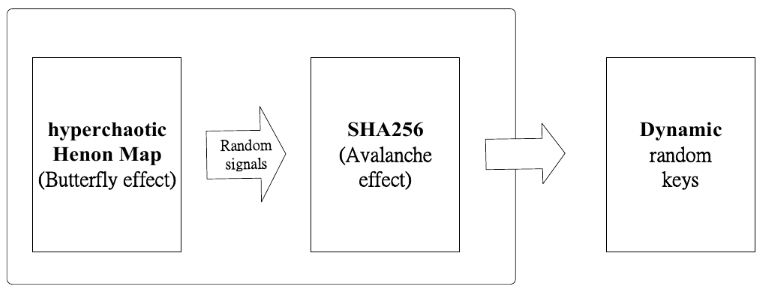
\includegraphics[width=350px]{chapters/res/chapter-2/img/lin.keygen.png}
  \caption{Ilustrasi proses pembangkitan kunci dinamis} \label{fig:lin.keygen}
  Sumber: \textcite{lin2021}
\end{figure}

Proses sinkronisasi sistem \emph{chaos} dapat dilakukan dengan mendekomposisi nilai $u(k)$ menjadi nilai $u_m(k)$ dan $u_s(k)$. Pemecahan nilai ini ditujukan untuk meningkatkan kemananan saat implementasi. Nilai $u_m(k)$ akan dikirimkan dari \emph{transmitter} menuju \emph{receiver}. Sistem ini dapat dijelaskan melalui gambar . Menurut \textcite{lin2021}, sistem itu aman. Hal ini dikarenakan apabla \emph{hacker} memiliki parameter-parameter yang digunakan untuk sinkronisasi, mereka tidak dapat mendapatkan \emph{state} dari master dan slave. Ilustrasi yang proses enkripsi dan dekripsi serta sinkronisasi yang dilakukan terdapat pada gambar \ref{fig:lin.caes}.

\begin{figure}[!h]
  \centering
  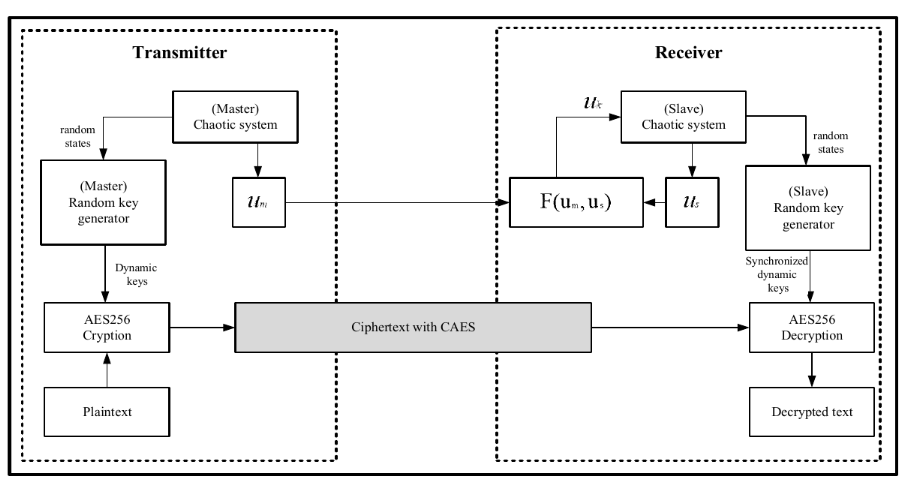
\includegraphics[width=350px]{chapters/res/chapter-2/img/lin.caes.png}
  \caption{Arsitektur AES berbasis \emph{chaos} yang telah diimporvisasi} \label{fig:lin.caes}
  Sumber: \textcite{lin2021}
\end{figure}

Pengujian dari sistem yang dilakukan oleh \textcite{lin2021} adalah dengan cara membandingkan proses enkripsi gambar yang dihasilkan memanfaatkan AES-ECB, AES-CBC, dan CAES-EBC. gambar yang diuji merupakan gambar berukuran $256 \times 256$. Pada algoritma CAES, kunci dinamis yang dihasilkan sebanyak 49.152 kunci. Setiap kunci ini dibuat secara langsung melalui proses \emph{update} pada setiap \emph{round} enkripsi. Hasil enkripsi pada gambar \ref{fig:lin.result} menunjukan bahwa CAES-ECB bila diobservasi secara visual memiliki kualitas yang cukup baik bila dibandingkan dengan AES-EBC. Menurut \textcite{lin2021}, Hal ini dapat membuktikan bahwa algoritma CAES-CBC lebih unggul dibandingkan AES-EBC dan AES-CBC.

\begin{figure}[!h]
  \centering
  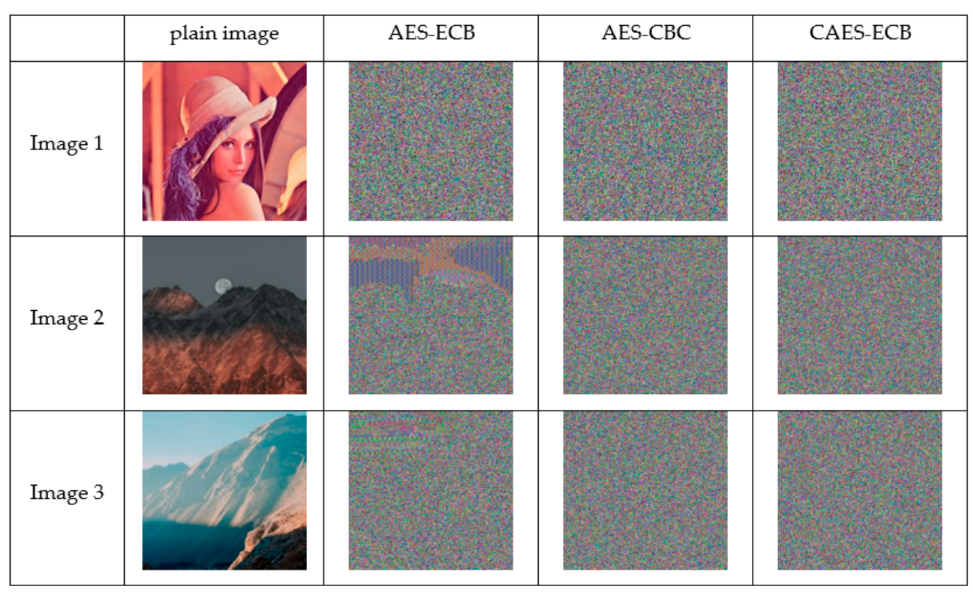
\includegraphics[width=350px]{chapters/res/chapter-2/img/lin.res.png}
  \caption{Hasil visual gambar terenkripsi} \label{fig:lin.result}
  Sumber: \textcite{lin2021}
\end{figure}

Proses enkripsi tersebut juga dilakukan proses pengujian secara analitik. Tes yang dilakukan berdasarkan parameter uji yang telah didefinisikan oleh National Institute of Standards and Technology (NIST). Pengujian yang dilakukan oleh \textcite{lin2021} menggunakan data \emph{stream} sepanjang 10.000.000 bit data dengan jumlah biat setiap stream sebesar 30. Hasil tersebut menunjukan bahwa algoritma CAES memenuhi persyaranan NIST SP 800-22 \emph{random number detection}. Hasil dari pengujian NIST juga menunjukan bahwa algoritma CAES lebih unggul dibandingkan dengan AES-CBC dan AES-EBC. Hal ini ditunjukan dengan data pada gambar \ref{fig:lin.analytic-result}.

\begin{figure}[!h]
  \centering
  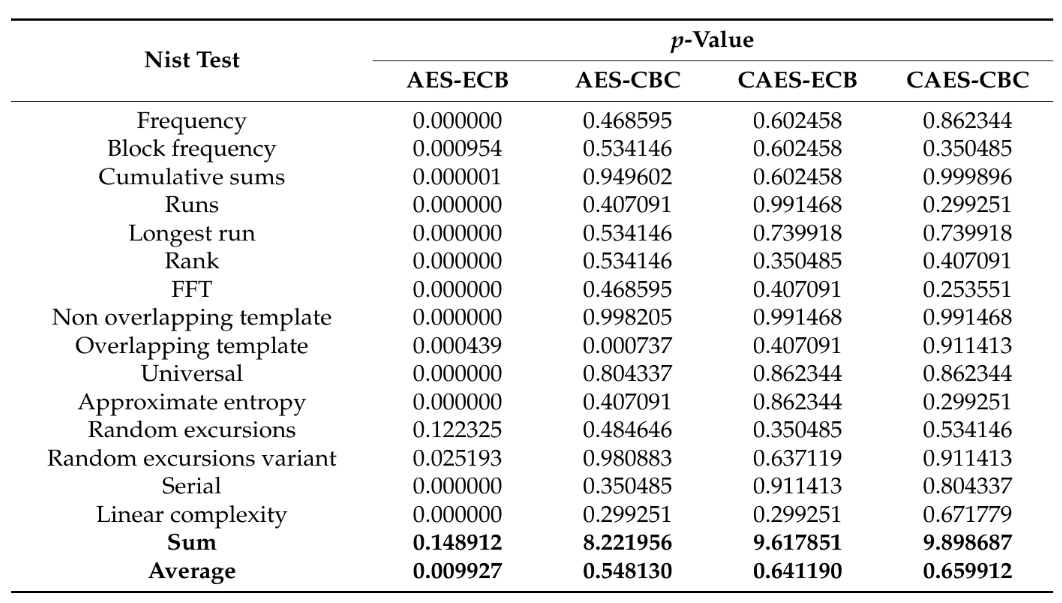
\includegraphics[width=350px]{chapters/res/chapter-2/img/lin.analytic-test.png}
  \caption{Hasil Analitik Algoritma CAES} \label{fig:lin.analytic-result}
  Sumber: \textcite{lin2021}
\end{figure}

\subsection{Enkripsi gambar dan Analisisnya memanfaatkan Algoritma AES dinamis}

Pada penelitian yang dilakukan oleh \textcite{singh2019}, kedinamisan proses enkripsi dilakukan pada S-box. Pada penelitian ini, S-box yang dimiliki oleh AES akan dipermutasi. Terdapat tiga parameter yang digunakan dalam pembentukan S-box ini, yaitu sebagai berikut:
\begin{enumerate}
  \item Kunci\\ Kunci sangat berpengruh terhadap hasil S-box yang dibentuk. Perubahan kecil pada kunci perlu menyebabkan S-box keluaran yang jauh berbeda.
  \item \emph{Irreducible polynomial}\\ Pada penelitian yang dilakukan oleh \textcite{singh2019}, pemilihan \emph{Irreducible polynomial} dilakukan secara acak. Hal ini berbeda dengan algoritma AES pada umumnya yang hanya menggunakan satu polinomial yang digunakan untuk membentuk S-box.
  \item Konstanta Affine\\ Konstanta affine yang digunakan dalam pembentukan S-box. Terdapat 256 konstanta yang dapat digunakan. Dalam penelitian yang dilakukan \textcite{singh2019}, semua konstanta yang dapat digunakan dipilih secara acak untuk membentuk S-box.
\end{enumerate}

Menurut \textcite{singh2019}, S-box yang dapat dibentuk sangat sensitif terhadap tiga parameter diatas. Dengan menggunakan metode tersebut, jumlah kemungkinan S-box dinamis yang dapat dibentuk adalah $256!$. Hal ini dapat memberikan tambahan keamanan pada cipherteks dikarenakan kerumitan tidak hanya berada pada kunci tetapi terdapat pada algoritma.

Pada penelitian \textcite{singh2019}, algoritma enkripsi yang telah dijelaskan sebelumnya diuji dengan melakukan enkripsi gambar \emph{grayscale}. Pengujian yang dilakukan adalah pengujian analisis histogram, pengujian korelasi koefisien, kualitas enkripsi, entropi informasi, dan NPCR-UACI test. Hasil pengujian menunjukan bahwa AES dan Dynamic AES memiliki kualitas enkripsi yang cukup setara. Akan tetapi, dalam pengujian korelasi koefisien, AES dinamis memiliki hasil yang lebih baik dibandingkan dengan AES.

\subsection{Perbaikan Keamanan dari Algoritma AES memanfaatkan \emph{Salt} Dinamis}

Pada penelitian yang dilakukan oleh \textcite{bachtiar2018}, proses enkripsi dinamis dilakukan dengan cara menambahkan \emph{salt} pada pesan yang akan dienkripsi. Nilai \emph{salt} dibuat berdasarkan hasil dari algortima \emph{Linear Congruental Generator} (LCG). Secara global, proses enkripsi dilakukan dengan melakukan proses enkripsi dinamis terlebih dahulu. Setelah itu, proses enkripsi akan dilakukan dengan melakukan AES pada pesan yang telah dilakukan enkripsi dinamis. Proses ini dapat digambarkan pada gambar \ref{fig:bachtiar.enc.process}.

\begin{figure}[!h]
  \centering
  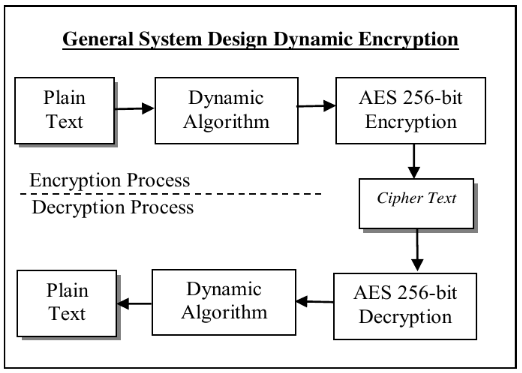
\includegraphics[width=250px]{chapters/res/chapter-2/img/bachtiar.enc.process.png}
  \caption{Ilustrasi proses pembangkitan kunci dinamis} \label{fig:bachtiar.enc.process}
  Sumber: \textcite{bachtiar2018}
\end{figure}

Pada proses enkripsi dinamis, akan dihitung \emph{salt} berdasarkan waktu. Nilai \emph{salt} akan dibuat melalui algoritma LCG.  Nilai salt ini akan ditambahkan pada pesan. Setelah pesan ditambahkan dengan \emph{salt}, pesan akan dilakukan proses enkripsi terlebih dahulu menggunakan OTP. Kunci yang digunakan untuk melakukan OTP merupakan kunci yang sama yang akan digunakan pada proses enkripsi menggunakan AES. Setelah proses ini dilakukan, pesan dinamis tersebut akan dienkripsi menggunakan AES.

Berdasarkan hasil pengujian yang dilakukan menggunakan NIST, teknik memanfaatkan pesan dinamis memberikan hasil yang lebih baik dibandingkan dengan tanpa menggunakan \emph{salt} atapun dengan hanya memanfaatkan \emph{salt} saja. Teknik memanfaatkan pesan dinamis untuk melakukan enkripsi secara dinamis memberikan nilai keberhasilan sebesar $72.5\%$. Nilai keberhasilan ini diperoleh berdasarkan pengujian dengan menjalankan sebanyak delapan kali dan dilakukan perhitungan secara rata-rata.

% ---------------------------------------------------%
% DISCLAIMER: ADA KEMUNGKINAN BAB 3 STRUKTUR YG DIBAHAS BERBEDA, JADI DI BAWAH ADA CONTOH
% BAB 3 KATING. MODIF SAJA SESUAI KEBUTUHAN

% ---------------------------------------------------%

% \chapter{Analisis dan Perancangan}
\chapter{Analisis Masalah dan Solusi}

\section{Analisis Masalah}
\label{sec:analisis-masalah}

Protokol komunikasi pada dasarnya dibangun untuk melayani komunikasi data antara dua buah pihak yang berbeda. Hal ini sesuai syarat jaringan komputer yang telah dijelaskan pada bagian \ref{sec:jaringan-komputer}. Protokol komunikasi harus dapat memastikan pesan yang dikirimkan dapat diterima oleh pihak penerima pesan serta dipahami isinya. Selain itu, protokol komunikasi juga harus memastikan ancaman apabila terdapat pihak ketiga yang terlibat baik secara aktif ataupun pasif. Selain itu, penerapan enkripsi dinamis pada sistem \emph{chaos} menimbulkan beberapa masalah kompatibilitas. Oleh karena itu, terdapat beberapa permasalahan yang akan dibahas pada bagian ini. Secara garis besar, permasalahan yang muncul ditunjukan pada tabel \ref{tab:permasalahan}.

\begin{table}[!h]
  \centering
  \caption{Permasalahan yang dihadapi pada protokol TLS dengan \emph{Cipher} berbasis sistem \emph{chaos}} \label{tab:permasalahan}
  \begin{tabular}{|c|p{6cm}|p{4cm}|}
    \hline
    \textbf{ID Masalah} & \textbf{Deskripsi} & \textbf{Rumusan Masalah Terkait} \\
    \hline
    P1 & Pemilihan Versi Protokol TLS & 2 \\ \hline
    P2 & Serangan MITM saat adanya komunikasi berlangsung & 2 \\ \hline
    P3 & Serangan \emph{replay attack} saat adanya komunikasi berlangsung & 1 dan 2 \\ \hline
    P4 & Serangan \emph{tampering} pada pesan terenkripsi & 2 \\ \hline
    P5 & Serangan kriptografi melalui analisis pesan terenkripsi & 1 \\ \hline
    P6 & Ancaman analisis nilai acak yang dihasilkan oleh sistem \emph{chaos} & 1 \\ \hline
    P7 & Pembentukan nilai awal sistem \emph{chaos} & 1 dan 2 \\ \hline
    P8 & Pembentukan kunci blok baru saat proses enkripsi dan dekripsi & 1 dan 2 \\ \hline
  \end{tabular}
\end{table}

\subsection{Ancaman Keamanan pada Protokol Komunikasi}
\label{sec:ancaman-keamanan}

Pihak ketiga mungkin terlibat dalam komunikasi baik secara aktif maupun pasif. Hal ini dapat menimbulkan beberapa ancaman keamanan yang ada pada protokol komunikasi. Bagian ini akan menjelaskan rincian analisis ancaman keamanan yang dihadapi oleh protokol ini. Untuk mempermudah penjelasan, diasumsikan terdapat dua buah pihak yang melakukan komunikasi, yaitu Ahmad dan Budi. Terdapat pihak ketiga dalam komunikasi bernama Candra sebagai pihak yang tidak berhak terlibat dalam komunikasi. 

Dalam komunikasi, memungkinkan Candra mengaku sebagai salah satu pihak yang terlibat dalam komunikasi, yaitu Ahmad dan Budi. Hal ini dapat dilakukan dengan melakukan serangan MITM di antara kedua belah pihak. Dengan melakukan serangan ini, memungkinkan Candra mendapatkan informasi yang dikirimkan oleh Ahmad dan Budi. Oleh karena itu, perlu adanya mekanisme untuk memastikan bahwa pihak yang terlibat merupakan pihak yang dipercaya.

Selain itu, Candra juga dapat melakukan serangan berupa \emph{replay attack}. Dalam serangan ini, Candra bertujuan untuk mengganggu sistem dengan mengirimkan ulang pesan-pesan tertentu yang telah direkam. Candra mungkin tidak dapat mengetahui isi dari data yang ada pada \emph{frame}, tetapi \emph{frame} tersebut dapat menyebabkan efek yang tidak diinginkan oleh Ahmad ataupun Budi. Oleh karena itu, perlu adanya otentikasi partisipan pada pesan.

Dalam komunikasi, Candra dapat mengubah \emph{frame} yang dikirimkan oleh Ahmad ataupun Budi. Hal ini dapat menyebabkan pesan yang dikirimkan tidak dapat dipahami oleh penerima. Selain itu, hal ini dapat memberikan efek yang tidak diinginkan oleh penerima, seperti serangan \emph{bit flip}. Oleh karena itu, perlu adanya mekanisme untuk menjaga integritas pesan yang dikirimkan oleh Ahmad ataupun Budi.

Pesan yang dikirimkan dalam jaringan publik dapat diamati oleh Candra. Candra dapat mengetahui isi pesan terenkripsi yang telah dikirimkan oleh Ahmad ataupun Budi. Hal ini dapat dicapai dengan melakukan beberapa teknik diantaranya adalah melakukan \emph{brute force} terhadap kunci enkripsi. Teknik lainnya yang dapat dilakukan oleh Candra adalah melakukan analisis teks enkripsi. Salah satu teknik yang bisa dilakukan adalah melakukan analisis berbasiskan \emph{plaintext} yang telah diketahui. Candra dapat mengamati pola yang dibentuk dari hasil enkripsi. Candra juga dapat melakukan analisis terhadap \emph{ciphertext} yang telah diterima. Hal ini dapat dilakukan dengan melakukan analisis frekuensi terhadap blok pesan ataupun melakukan analisis secara visual terhadap \emph{ciphertext}. Harapan dari proses ini mendapatkan pola dari \emph{ciphertext} sehingga dapat dianalisis apa isi pesan yang terenkripsi.

\subsection{Analisis Permasalahan Penerapan AES dengan Sistem \emph{Chaos} pada Protokol TLS}
\label{sec:ancaman-implementasi}
Dalam penerapan \emph{cipher} AES dengan sistem \emph{chaos} pada protokol TLS, diperlukan memilih versi protokol TLS yang tepat. Pemilihan versi protokol TLS yang tepat perlu memperhatikan keamanan yang diberikan oleh protokol tersebut. Pada dasarnya, protokol TLS memiliki beberapa versi yang berbeda, diantaranya adalah TLSv1.0, TLSv1.1, TLSv1.2, dan TLSv1.3. 

Selain itu, sistem \emph{chaos} yang tepat perlu dipilih untuk digunakan sebagai kunci blok. Sistem \emph{chaos} ini juga harus memiliki sifat \emph{forward unpredictability} dan \emph{backward unpredictability} sebagaimana yang dijelaskan pada bagian \ref{sec:nist.statistical.test}. Ancaman yang terkait dengan hal ini adalah adanya analisis nilai acak untuk mendapatkan nilai acak yang akan datang dan nilai acak yang telah digenerate sebelumnya. Hal ini dapat menyebabkan pesan yang dikirimkan dapat didekripsi oleh penyerang, baik pesan yang diterima dan pesan yang akan datang.

Sistem \emph{chaos} juga memerlukan nilai awal atau \emph{seed} yang akan digunakan sebagai nilai awal dari sistem \emph{chaos}. Nilai ini perlu dihasilkan dari proses \emph{handshake} yang dilakukan melalui protokol TLS. Oleh karena itu, diperlukan sebuah mekanisme pembangkitan nilai \emph{seed} melalui prosedur \emph{handshake} tersebut.

Pada protokol TLS berbasis chaos, kunci blok yang digunakan bersifat dinamis. Hal ini memerlukan analisis lebih lanjut terkait metode pembaruan kunci blok yang digunakan pada protokol ini pada masing-masing pihak. Hal ini diperlukan agar \emph{state} dari kunci blok dapat terjamin.

Pada protokol TLS, terdapat mekanisme pemeriksaan integritas pesan. Mekanisme ini memanfaatkan MAC yang dienkripsi bersama pesan. Ancaman dari mekanisme ini adalah adanya serangan dengan mengirimkan pesan yang tidak sah. Pembangkitan nilai acak pada sistem \emph{chaos} dinilai cukup berat sehingga bila ancaman ini terjadi, penerima dapat kehabisan \emph{resource} dalam melakukan dekripsi. Oleh karena itu, perlu adanya mekanisme untuk melakukan mekanisme pemeriksaan integritas pesan yang diterima yang lebih efisien.

\section{Analisis Solusi}

Bagian ini akan menjelaskan terkait solusi dari permasalahan yang telah dipaparkan sebelumnya. Bagian ini akan dibagi menjadi beberapa kategori, diantaranya adalah solusi terkait dengan proses sistem chaos, sinkronisasi sistem chaos, proses enkripsi dan dekripsi, dan proses otentikasi pengirim pesan. Secara garis besar, solusi yang diusulkan ditunjukkan pada tabel \ref{tab:solusi}.

\begin{table}[!h]
  \centering
  \caption{Solusi yang diusulkan pada protokol yang diusulkan} \label{tab:solusi}
  \begin{tabular}{|c|p{6cm}|c|}
    \hline
    \textbf{ID Solusi} & \textbf{Deskripsi} & \textbf{Permasalahan Terkait} \\
    \hline
    S1 & Menggunakan sistem chaos berbasis \emph{Sine-Henon map} untuk pembangkit bilangan acak & P5 dan P6 \\ \hline
    S2 & Pertukaran Kunci menggunakan Diffie-Hellman & P7 \\ \hline
    S3 & Proses pembangkitan \emph{state} awal sistem \emph{chaos} dilakukan dari proses TLS Handshake & P7 \\ \hline
    S4 & Cipher yang digunakan adalah AES dengan blok CTR dan kunci blok dinamis berbasiskan sistem chaos \emph{Sine-Henon map} & P3 dan P5 \\ \hline
    S5 & Mekanisme pengubahan kunci enkripsi dan dekripsi & P8 \\ \hline
    S6 & Pesan terenkripsi dilindungi oleh MAC yang melibatkan nomor frame & P4 \\ \hline
    S7 & Parameter Diffie-Hellman harus ditandatangani melalui tanda tangan digital & P2 \\ \hline
    S8 & Mekanisme pemeriksaan tanda tangan digital & P2 \\ \hline
    S9 & Melakukan implementasi pada protokol TLSv1.2 & P1, P2, P4, dan P4 \\ \hline
    S10 & Melakukan implementasi pemeriksaan \emph{certificate} pada sisi klien & P2 \\ \hline
  \end{tabular}
\end{table}

\subsection{Sistem Chaos}

Pada penelitian yang dilakukan oleh \textcite{lin2021}, sistem chaos yang digunakan adalah sistem chaos berbasis Hénon Map. Nilai hasil pembangkitan diambil melalui parameter $X_n$ yang dihasilkan pada setiap iterasi. Bila diamati melalui persamaan \ref{eq:chaos.henon}, bila diketahui nilai $X_n$, akan sangat sulit untuk mendapatkan nilai $X_{n-1}$ dikarenakan diperlukannya nilai $Y_n$ yang tidak diketahui. Oleh karena itu, sistem chaos ini sukar untuk dilakukan \emph{backward predictability}. Kelemahan dari sistem \emph{chaos} ini adalah sistem ini masih dapat dilakukan \emph{forward predictability} bila dua nilai berurutan yang dihasilkan oleh sistem \emph{chaos} dapat diketahui. 

Hal ini dapat diperbaiki dengan melibatkan sistem chaos lain berbasis \emph{sine map}. Sistem chaos berbasis \emph{sine map} dipilih dikarenakan sistem chaos ini menghasilkan titik diantara $0$ dan $1$ sehingga memudahkan dalam melakukan konversi dalam byte. Selain itu, nilai diantara $0$ dan $1$ juga memiliki kepadatan yang cukup baik bila diinterpretasikan pada \emph{floating point} sehingga diharapkan dapat menghasilkan nilai acak yang lebih banyak.

Peraduan antara sistem chaos berbasis \emph{sine map} dan sistem chaos berbasis Hénon Map dapat dilakukan seperti metode yang dijelaskan oleh \textcite{patel2021}. Dari hasil tersebut, dapat dibentuk sistem \emph{chaos} baru yang disebut SineHenonMap yang didefinisikan pada persamaan \ref{eq:tls.chaos}.

\begin{equation}
  \begin{aligned}
    X_{i+1} = \text{mod}((1 - a \cdot X_i^2 + Y_i) + (\frac{\mu}{4} \cdot \sin{(\pi \cdot X_{i})}) \cdot 100, 1)  \\
    Y_{i+1} = \text{mod}((b \cdot X_i + Z_{i}) \cdot 100, 1) \\
    Z_{i+1} = \frac{\mu}{4} \cdot \sin{(\pi \cdot Z_{i})}
  \end{aligned}
  \label{eq:tls.chaos}
\end{equation}

Pada persamaan \ref{eq:tls.chaos}, terdapat pengali dengan nilai $100$. Nilai ini digunakan untuk memperoleh distribusi \emph{uniform} pada nilai yang dihasilkan sebagaimana yang dilakukan oleh \textcite{nurhaliza2023}. Hal ini diilustrasikan pada gambar \ref{fig:chaos.sinehenonmap.dist}. Pemilihan nilai $\mu$ yang digunakan adalah $3.75$ dan $a$ serta $b$ adalah $1.4$ dan $0.3$. Hal ini diambil berdasarkan nilai yang digunakan pada penelitian \textcite{lin2021} dan \textcite{patel2021}. Prasyarat dari sistem chaos pada persamaan \ref{eq:tls.chaos} adalah nilai $X_0$, $Y_0$, dan $Z_0$ harus berada pada range $(0,1)$. Hal ini dilakukan untuk menjamin kepadatan nilai yang dihasilkan oleh sistem \emph{chaos}.

\begin{figure}[!h]
  \centering
  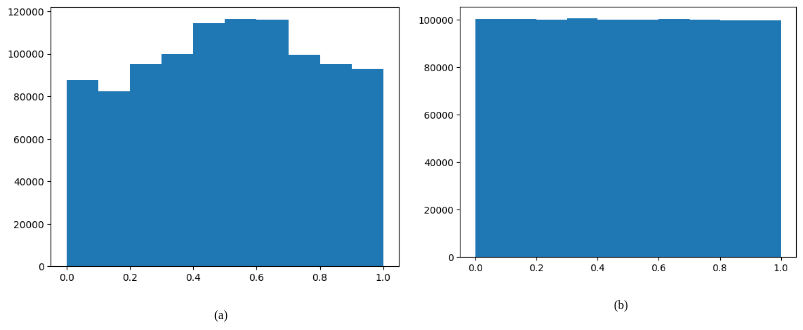
\includegraphics[width=400px]{chapters/res/chapter-3/img/sinehenon.distribution.png}
  \caption{Distribusi nilai dari sistem chaos Sine-Hénon Map (a) tanpa pengali dan (b) dengan pengali} \label{fig:chaos.sinehenonmap.dist}
\end{figure}

\subsection{Sinkronisasi Sistem Chaos}

Menurut \textcite{lin2021}, sinkronisasi sistem \emph{chaos} dapat dilakukan dengan memanfaatkan \emph{sliding mode control}. Namun, metode ini memerlukan RTT yang cukup banyak untuk melakukan sinkronisasi. Pada protokol TLS, pada dasarnya telah disediakan mekanisme untuk pertukaran kunci dengan melalui proses \emph{handshake}. Oleh karena itu, sinkronisasi sistem \emph{chaos} dapat dilakukan dengan memanfaatkan \emph{master key} dari proses tersebut.

Permasalahan selanjutnya adalah terkait dengan konversi nilai bilangan bulat menjadi nilai \emph{state} pada sistem \emph{chaos}. Prasayat dari sistem \emph{chaos} pada persamaan \ref{eq:tls.chaos} adalah nilai $X_0$, $Y_0$, dan $Z_0$ harus berada pada range $(0,1)$. Oleh karena itu, proses konversi dapat dilakukan dengan melakukan ekspansi kunci setidaknya $3n$ bit nilai. Selanjutnya, nilai tersebut dilakukan perbandingan nilai pada blok hasil ekspansi kunci dengan nilai maksimum blok tersebut. Hal ini dinyatakan pada persamaan \ref{eq:tls.convert}.

\begin{equation}
  \begin{aligned}
    f(K) = \frac{K}{2^{n}} \\
  \end{aligned}
  \label{eq:tls.convert}
\end{equation}

Dalam hal ini nilai $n$ adalah jumlah bit maksimum. Pada protokol yang dibangun, jumlah bit yang diambil adalah $n = 256$. Hal ini didasari dengan tipe data float memiliki ketelitian yang cukup baik pada 32 bit.

Protokol TLS pada dasarnya mendukung dua tipe pertukaran kunci seperti yang telah dijelaskan pada \emph{sec:tls.keyexchange}. Pertukaran kunci yang cocok untuk diterapkan pada sistem \emph{chaos} adalah pertukaran kunci dengan memanfaatkan protokol Diffie-Hellman. Hal ini dikarenakan protokol ini memiliki keamanan yang lebih tinggi dibandingkan RSA. Selain itu, keteracakan dihasilkan juga oleh kedua buah pihak yang terlibat sehingga keteracakan tidak hanya tergantung oleh satu pihak. Hal ini sesuai dengan prinsip \emph{defense in depth} pada keamanan data.


\subsection{Enkripsi dan Dekripsi Pesan}
\label{sec:solusi.enc-dec}

Pada saat proses enkripsi ataupun dekripsi pesan, diperlukan bit-bit kunci yang dibangkitkan melalui sistem \emph{chaos}. Proses pengubahan titik \emph{chaos} pada persamaan \ref{eq:tls.chaos} menjadi bilangan bulat dapat dilakukan persamaan \ref{eq:tls.convert.int}.

\begin{equation}
  \begin{aligned}
    K_i = \lfloor{X_i \cdot 2^{n}}\rfloor
  \end{aligned}
  \label{eq:tls.convert.int}
\end{equation}

Proses pengubahan ini diambil dikarenakan $K_i$ yang dihasilkan akan langsung berada pada jumlah bit yang dibutuhkan. Hal ini dapat menghemat operasi yang diperlukan dalam melakukan konversi. Nilai $K_i$ yang dihasilkan akan digunakan sebagai kunci blok yang digunakan pada proses enkripsi dan dekripsi.

Algoritma yang digunakan untuk proses enkripsi dan dekripsi adalah AES-256. Algoritma enkripsi ini dikarenakan dukungan terhadap algoritma ini sudah sangat baik pada berbagai sistem. Selain itu, kekuatan dari AES-256 sampai saat ini masih sangat baik. Algoritma ini juga dapat dijalankan pada berbagai perangkat dengan kecepatan yang baik dengan adanya bantuan microprocessor yang mendukung instruksi AES.

Permasalahan selanjutnya adalah terkait dengan sistem blok yang digunakan. Pada protokol yang dibangun, sistem blok yang digunakan adalah mode CTR. Mode CTR dapat memberikan fleksibilitas dalam pembentukan kunci dikarenakan proses enkripsi dan dekripsi keduanya dapat dilakukan secara paralel. Selain itu, mode CTR dapat diubah dengan mudah menjadi \emph{cipher} alir sehingga dapat digunakan untuk mengirimkan aliran pesan yang terenkripsi. Mode sistem CTR juga dapat mengaburkan hubungan antar blok dikarenakan blok akan dienkripsi dengan blok CTR yang berbeda-beda.

Nilai \emph{counter} pada sistem blok CTR dibangun juga memanfaatkan sistem \emph{chaos}. Hal ini ditujukan untuk menambah keamanan dari enkripsi blok. Selain itu, menambahan sistem \emph{counter} ini juga memperpanjang orde dari kunci yang digunakan. Hal ini dapat memperbesar ruang kunci saat melakukan XOR. Oleh karena itu, upaya analisis terhadap pesan akan semakin sulit.

Permasalahan terkait dengan pembaruan kunci blok dapat diselesaikan dengan memberikan aturan terkait dengan pembaruan kunci. Untuk kunci enkripsi, pembaruan kunci dilakukan setelah proses enkripsi berhasil. Hal ini cukup untuk dilakukan karena frame yang terenkripsi dapat dilakukan \emph{cache} apabila dibutuhkan retransmisi ulang. Selain itu, pembaruan kunci segera juga mencegah kunci yang digunakan untuk enkripsi diambil oleh penyerang untuk melakukan dekripsi pesan yang telah dienkripsi sebelumnya. Untuk pengubahan nilai \emph{counter}, dapat dilakukan setelah proses enkripsi selesai. Hal ini untuk memastikan nilai \emph{counter} berubah hanya saat proses enkripsi berhasil. 

Permasalahan selanjutnya adalah terkait dengan pengubahan nilai kunci saat proses dekripsi. Perubahan kunci hanya boleh dilakukan saat MAC pesan yang diterima benar dan proses dekripsi berhasil. Hal ini untuk memastikan bahwa pesan yang diterima merupakan pesan yang benar. Pengubahan nilai counter hanya boleh dilakukan saat proses dekripsi berhasil. Hal ini untuk memastikan bahwa nilai counter yang digunakan merupakan nilai yang benar. Saat melakukan proses dekripsi, nilai awal dari sistem \emph{chaos} harus disimpan terlebih dahulu. Hal ini diperlukan untuk melakukan operasi \emph{rollback} apabila terjadi kegagalan saat melakukan dekripsi.

Permasalahan selanjutnya adalah terkait kegagalan saat melakukan proses dekripsi pada pesan yang diterima. Kondisi ini terjadi dengan dua kemungkinan, yaitu nilai MAC salah dan padding pesan salah. Apabila pesan yang diterima memiliki nilai padding salah, maka proses dekripsi dapat langsung dibatalkan saja sehingga proses komunikasi masih dapat dilanjutkan. Apabila pesan yang diterima memiliki nilai MAC yang salah, nilai state enkripsi harus dipulihkan ke nilai sebelum melakukan operasi. Oleh karena itu, perlu adanya penanganan hal tersebut.

Permasalahan terkait dengan \emph{replay attack} pada dasarnya sudah teratasi dengan mekanisme MAC pada TLS. Pada protokol TLS, perhitungan nilai MAC didasari juga dengan nomor frame. Oleh karena itu, pesan sudah terlindungi dari ancaman tersebut.

Permasalahan terkait dengan integritas pesan telah terjamin dengan adanya MAC yang digunakan. MAC dapat memastikan bahwa pesan yang diterima merupakan pesan yang asli dan otentik. Oleh karena itu, permasalahan terkait dengan integritas pesan telah teratasi.

\subsection{Otentikasi Pengirim Pesan}

Pada protokol TLS, telah terdapat mekanisme otentikasi pengirim pesan. Mekanisme ini dilakukan saat proses \emph{handshake} dan juga saat proses pengiriman berlangsung. Pada proses \emph{handshake}, terdapat proses penandatanganan digital pada parameter pertukaran kunci. Hal ini menjamin bahwa pihak yang dapat menghasilkan kunci hanyalah pihak yang benar. Penandatanganan parameter pertukaran kunci juga dapat mencegah adanya MITM attack karena nilai parameter pertukaran tersebut akan dapat diketahui apabila terjadi pengubahan.

Tanda tangan digital tersebut dibuktikan dengan data terkait sertifikat digital yang dikirimkan. Hal ini memastikan hanyalah pihak yang otentik saja yang dapat menghasilkan tanda tangan tersebut. Hal ini dijamin dengan adanya tanda tangan dari CA yang dipercaya oleh kedua belah pihak. Selama CA belum melakukan upaya \emph{revocation} ataupun sertifikat tidak kadaluarsa, maka tanda tangan tersebut dapat dipercaya berasal dari pihak yang sesungguhnya.

Sertifikat digital yang digunakan pada protokol ini adalah sertifikat digital yang dikeluarkan oleh CA yang dipercaya oleh kedua belah pihak. Sertifikat digital perlu diperiksa oleh \emph{client} untuk memastikan tidak adanya serangan MITM yang berlangsung. Pihak \emph{client} dapat juga menanam sertifikat yang dipercaya. Teknik ini akan menambah keamanan dari serangan MITM yang mungkin terjadi. 

Pada proses pengiriman pesan, terdapat mekanisme otentikasi pengirim pesan melalui MAC. MAC yang digunakan pada protokol ini bersifat dinamis. Hal ini dapat mencegah adanya MITM attack serta dapat memberikan nirpenyangkalan yang lebih tinggi dikarenakan partisipan yang terlibat dari awal komunikasi saja yang dapat menghasilkan MAC yang benar. Hal ini dikarenakan selain dibutuhkannya nilai awal dari sistem \emph{chaos}, diperlukan juga urutan frame saat ini untuk dapat menghasilkan MAC yang benar.

Pada MAC dan tanda tangan digital, digunakan fungsi hash SHA-2 dengan \emph{digest size} 256. Hal ini dikarenakan fungsi hash ini merupakan fungsi hash yang cukup umum digunakan. Selain itu, hingga saat ini fungsi hash masih belum ditemukan kerentanannya.

\section{Protokol TLS berbasis Chaos} \label{sec:protokol-tls-chaos}

Bagian ini menjelaskan terkait spesifikasi dari protokol TLS berbasis chaos yang akan dibangun. Bagian ini terbagi atas beberapa bagian, yaitu spesifikasi \emph{cipher}, spesifikasi \emph{handshake}, spesifikasi terkait dengan pengiriman pesan. Pada dasarnya, protokol yang dibangun akan mengikuti spesifikasi yang telah ada pada protokol TLSv1.2. Versi ini dipilih dikarenakan TLS versi ini masih dapat mendukung \emph{cipher} berbasis AEAD. Namun, terdapat beberapa penyesuaian yang dilakukan untuk memastikan kompatibilitas dari protokol yang dibangun.

\subsection{Spesifikasi Cipher}

\emph{Cipher} yang digunakan pada protokol ini adalah AES-256. Kunci enkripsi serta nilai \emph{counter} yang digunakan pada \emph{cipher} ini bersifat dinamis memanfaatkan sistem chaos yang telah dijelaskan pada bagian \ref{sec:solusi.enc-dec}. Mode blok yang digunakan pada \emph{cipher} ini adalah counter. Gambar \ref{fig:tls.cipher} menunjukkan struktur enkripsi dan dekripsi dari \emph{cipher} yang digunakan.

\begin{figure}[!h]
  \centering
  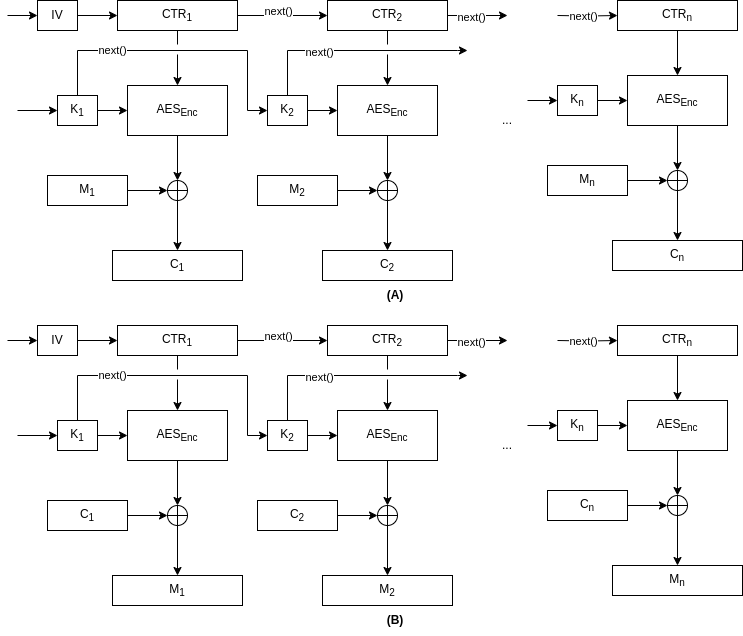
\includegraphics[width=\textwidth]{chapters/res/chapter-3/img/cipher.png}
  \caption{Ilustrasi Sistem Chaos untuk (A) Enkripsi (B) Dekripsi} \label{fig:tls.cipher}
\end{figure}

Nilai $IV$ dan $K1$ keduanya diinisialisasi berdasarkan hasil dari pertukaran kunci. Metode $\text{next}(\cdot)$ merupakan metode untuk memperbaharui sistem chaos berdasarkan persamaan \ref{eq:tls.chaos}.

Kunci MAC yang digunakan adalah kunci statis. Proses perhitungan MAC perlu melibatkan nomor frame yang digunakan sebagaimana solusi S6. Perhitungan MAC dilakukan sesuai dengan persamaan \ref{eq:tls.data.mac}.

\begin{equation}
  \label{eq:tls.data.mac}
  \begin{array}{l}
    H = \text{HMAC}(\text{key}, \text{frame\_number}\text{ }|| \\ 
      \text{   }\text{frame}.\text{type}\text{ }|| \\
      \text{   }\text{frame}.\text{version}\text{ }|| \\ 
      \text{   }\text{frame}.\text{length}\text{ }|| \\
      \text{   }\text{frame}.\text{plaintext} \\
    ) 
  \end{array}
\end{equation}

Aturan untuk pembaruan kunci telah dijelaskan pada bagian \ref{sec:solusi.enc-dec}. Bila digambarkan melalui diagram \emph{sequence}, proses pembaruan kunci dapat dilihat pada gambar \ref{fig:tls.cipher.update.mac.write} dan \ref{fig:tls.cipher.update.mac.read}.


\begin{figure}[!h]
  \centering
  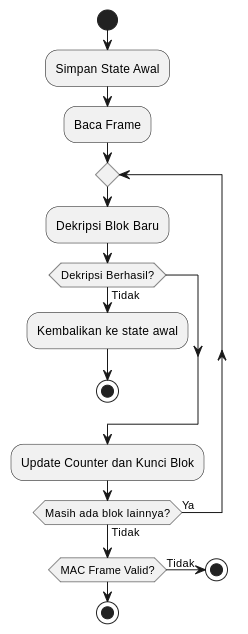
\includegraphics[width=200px]{chapters/res/chapter-3/img/update.write.png}
  \caption{Ilustrasi Proses Pembaharuan Kunci Dekripsi dan MAC pada Proses Pembacaan} \label{fig:tls.cipher.update.mac.read}
\end{figure}

\begin{figure}[!h]
  \centering
  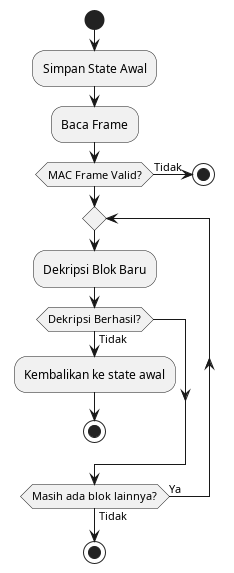
\includegraphics[width=200px]{chapters/res/chapter-3/img/update.read.png}
  \caption{Ilustrasi Proses Pembaharuan Kunci Enkripsi dan MAC pada Proses Penulisan} \label{fig:tls.cipher.update.mac.write}
\end{figure}

Pada proses enkripsi, pesan pada mulanya akan dipotong menjadi beberapa frame yang kecil. Setiap frame, akan dihitung nilai MAC dari frame tersebut lalu nilainya akan ditempelkan pada pesan. Selanjutnya, pesan akan dilakukan proses \emph{padding} dengan kelipatan 16 bytes. Hal ini agar sesuai dengan panjang blok enkripsi. Setelah pesan dilakukan \emph{padding}, tiap frame akan dilakukan operasi sebagaimana pada gambar \ref{fig:tls.cipher.update.mac.write}. Pesan yang berhasil dienkripsi akan disusun menjadi sebuah \emph{record} yang akan dikirimkan.

Pada saat menerima pesan, penerima akan melakukan proses dekripsi yang dilakukan sebagaimana pada gambar \ref{fig:tls.cipher.update.mac.read}. Setelah proses dekripsi berhasil, pesan akan dihitung MAC-nya. Bila nilai MAC valid, pesan akan digabungkan dan dilanjutkan ke \emph{layer} yang lebih tinggi. Hash yang digunakan pada MAC adalah SHA-256.

\emph{Cipher} yang dijelaskan pada bagian ini akan ditandai dengan kode \emph{cipher suite} $\text{0xff00}$ pada saat proses \emph{handshake}. Nilai awal $\text{0xff}$ berdasarkan \textcite{rfc5246} merupakan nilai yang privat sehingga dapat dijamin tidak akan bertabrakan dengan \emph{cipher suite} yang telah ada.

\subsection{Spesifikasi \emph{Handshake}}
Proses handshake dilakukan sebagaimana pada protokol TLS yang dijelaskan pada bagian \ref{sec:tls.handshake}. Proses ini dilakukan untuk membangkitkan \emph{master secret} yang digunakan. Terdapat beberapa spesifikasi khusus yang diterapkan pada protokol yang dibangun. Pertukaran kunci yang didukung hanyalah menggunakan Eliptic Curve Diffie-Hellman. Hal ini ditujukan agar keamanan dari \emph{premaster secret} dapat terjamin.

\begin{figure}[!h]
  \centering
  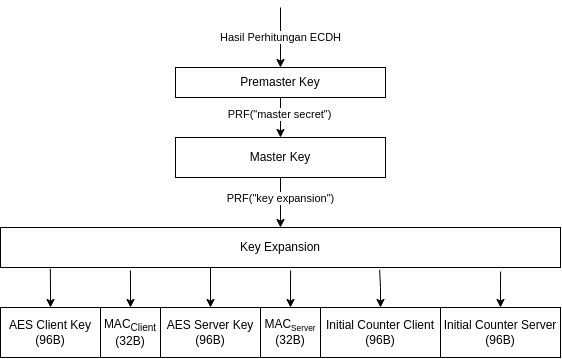
\includegraphics[width=400px]{chapters/res/chapter-3/img/keygen.png}
  \caption{Ilustrasi Pembangkitan Kunci} \label{fig:tls.keygen}
\end{figure}


Proses pembangkitan kunci diilustrasikan melalui gambar \ref{fig:tls.keygen}. Hasil dari proses Eliptic curve Diffie-Hellman akan menghasilkan \emph{premaster secret}. Saat \emph{premaster secret}, kunci \emph{master secret} akan dihasilkan melalui fungsi PRF. Saat \emph{master secret} berhasil dibangkitkan, perlu dilakukan proses \emph{key expansion}. Panjang kunci yang harus diekspansi adalah 448 bytes. Hal ini dikarenakan diperlukannya empat pasang sistem \emph{chaos} yang digunakan untuk pembangkitan sistem chaos dan dua buah kunci MAC. Tiap sistem \emph{chaos} memerlukan tiga buah parameter sehingga dibutuhkan 96 bytes per sistem \emph{chaos}. Ilustrasi dari ekspansi kunci dapat dilihat pada gambar \ref{fig:tls.keyexpansion}.

\begin{figure}[!h]
  \centering
  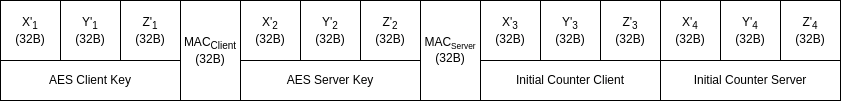
\includegraphics[width=400px]{chapters/res/chapter-3/img/keyexpansion.png}
  \caption{Ilustrasi Ekspansi Kunci} \label{fig:tls.keyexpansion}
\end{figure}

Persamaan \ref{eq:tls.key.convert} menunjukkan proses pengubahan kunci yang dilakukan menjadi parameter chaos. $K$ adalah potongan kunci dari hasil ekspansi.

\begin{equation}
  \begin{aligned}
    X_i = f(X'_i) \\
    Y_i = f(Y'_i) \\
    Z_i = f(Z'_i) \\
    E_i = (X_i, Y_i, Z_i)
  \end{aligned}
  \label{eq:tls.key.convert}
\end{equation}

Tabel \ref{tab:tls.keyexpansion} menunjukan kegunaan dari setiap hasil ekspansi kunci yang dilakukan. Tabel tersebut menjelaskan nilai awal dari sistem \emph{chaos} yang digunakan untuk pembangkitan kunci blok, kunci MAC, dan nilai IV.

\begin{table}[!h]
  \centering
  \caption{Parameter Hasil Ekspansi Kunci} \label{tab:tls.keyexpansion}
  \begin{tabular}{|p{3cm}|p{3cm}|p{6cm}|}
    \hline
    \textbf{Nama Parameter} & \textbf{Variabel} & \textbf{Deskripsi} \\
    \hline
    \emph{MAC Client Key} & $\text{MAC}_1$ & Nilai Kunci MAC yang digunakan oleh client \\ \hline
    \emph{MAC Server Key} & $\text{MAC}_2$ & Nilai Kunci MAC yang digunakan oleh server \\ \hline
    \emph{AES Client Key}  & $E_1$ & Nilai awal  parameter \emph{chaos} yang digunakan client untuk melakukan enkripsi ($K_1$) \\ \hline
    \emph{AES Server Key}  & $E_2$ & Nilai awal parameter \emph{chaos} yang digunakan server untuk melakukan enkripsi ($K_1$) \\ \hline
    \emph{Initial Counter Client}  & $E_3$ & Nilai \emph{counter} awal yang digunakan client untuk enkripsi \\ \hline
    \emph{Initial Counter Server}  & $E_4$ & Nilai \emph{counter} awal yang digunakan server untuk enkripsi \\
    \hline
  \end{tabular}
\end{table}

\subsection{Spesifikasi Pengiriman Pesan}

Pada proses pengiriman pesan, pesan terlebih dahulu dilakukan operasi kriptografi sebagaimana penjelasan pada bagian \ref{sec:solusi.enc-dec}. Setelah itu, pesan akan disusun menjadi sebuah \emph{record} yang akan dikirimkan. Gambar \ref{fig:tls.application.rec} menunjukkan protokol record yang digunakan untuk mengirimkan pesan.

\begin{figure}[!h]
  \centering
  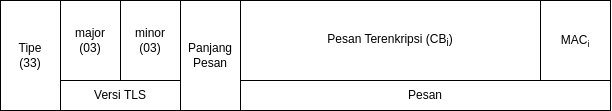
\includegraphics[width=\textwidth]{chapters/res/chapter-3/img/tls.application.record.png}
  \caption{Ilustrasi \emph{Application Record} yang digunakan} \label{fig:tls.application.rec}
\end{figure}

Berdasarkan \textcite{rfc5246}, Nilai tipe haruslah 33. Hal ini menyatakan bahwa pesan yang dikirimkan merupakan \emph{Application Data}. Nilai \emph{version} yang digunakan adalah $\text{0x0303}$. Hal ini menyatakan protokol yang digunakan adalah TLSv1.2. Panjang pesan ($L$) merupakan panjang dari pesan dan MAC dalam keadaan terenkripsi. Secara matematis dihitung berdasarkan persamaan \ref{eq:tls.record.length}.

\begin{equation}
  \begin{aligned}
    L = \text{len}(CB_{i})
  \end{aligned}
  \label{eq:tls.record.length}
\end{equation}

Blok pesan terenkripsi merupakan hasil dari proses enkripsi yang dilakukan pada bagian \ref{sec:solusi.enc-dec}. Blok tersebut berisi informasi terkait dengan \emph{plaintext} dan MAC dalam keadaan terenkripsi. Hal ini dilakukan untuk mencegah adanya serangan \emph{side-channel} dengan mengamati waktu dekripsi pesan.

\chapter{Implementasi dan Pengujian}

\section{Implementasi}

Bagian ini menjelaskan dari implementasi solusi yang telah dirancang sebelumnya. Bagian ini akan menjelaskan terkait lingkungan implementasi, batasan dari implementasi, serta implementasi tiap bagian dari protokol TLS.

\subsection{Batasan Implementasi}
Implementasi dilakukan dengan beberapa batasan dari protokol TLS yang telah didefinisikan pada \textcite{rfc5246}. Berikut ini merupakan batasan yang diterapkan:

\begin{enumerate}
  \item Implementasi hanya dilakukan menggunakan satdu \emph{cipher suite} saja, yaitu enkripsi menggunakan AES-256 berbasis sistem \emph{chaos}, pertukaran kunci ECDSA, algoritma hash SHA-256.
  \item Tiap pesan pada protokol \emph{handshake} dikirimkan melalui Protokol \emph{Record} yang berbeda.
  \item Fitur kompresi pada protokol TLS tidak diimplementasikan.
  \item Sertifikat digital diverifikasi secara \emph{pinning} dan tidak melakukan verifikasi \emph{revocation}.
  \item Sertifikat digital yang digunakan merupakan \emph{self-signed certificate} yang mendukung ECDSA untuk tanda tangan digital.
  \item Kurva eliptik yang didukung pada proses pertukaran kunci hanyalah kurva secp256r1.
\end{enumerate}
  
Pemilihan implementasi satu cipher ditujukan agar proses pengembangan dapat berfokus hanya pada \emph{cipher suite} yang hendak dikembangkan. Hal ini juga dapat membantu menyederhanakan pustaka yang dibangun sehingga proses pengembangan dapat lebih mudah dan cepat. 

Pemilihan pertukaran kunci berbasis ECDSA didasarkan pada kekuatan dari ECDSA. Menurut \textcite{munir2019}, ECDSA diyakini memiliki kekuatan yang setara dengan RSA walaupun dengan menggunakan kunci yang lebih pendek. Hal ini dapat membantu mengurangi \emph{resource} pada perangkat yang menggunakan pustaka ini.

Pengiriman pesan \emph{handshake} pada dasarnya dapat disatukan dalam sebuah protokol \emph{record}. Akan tetapi, pada implementasi pustaka ini, pesan \emph{handshake} dikirimkan terpisah dengan tujuan  membantu pada fase \emph{debugging} melalui aplikasi Wireshark dikarenakan tiap layer protokol \emph{record} akan ditampilkan secara terpisah.

Pada implementasi, fitur kompresi dinonaktifkan. Hal ini dikarenakan untuk melihat kualitas dari hasil enkripsi pada layer TLS. Kualitas yang dapat terlihat salah satunya terkait dengan hubungan antar blok serta keteracakan dari hasil enkripsi. Apabila plainteks dikomporesi, hasil enkripsi akan lebih mampat sehingga keteracakan akan sangat terlihat dan hilangnya hubungan antar blok.

Sertifikat digital yang digunakan pada implementasi ini merupakan sertifikat yang \emph{self-signed}. Fokus utama dari implementasi sertifikat digital hanya untuk memastikan bahwa MITM tidak terjadi. Oleh karena itu, implementasi berbentuk \emph{pinning} dan \emph{self-signed certificate} dinilai sudah cukup.

\subsection{Lingkungan Implementasi}

Lingkungan implementasi dari protokol TLS ditunjukan pada tabel \ref{tab:impl.env}.

\begin{table}[!h]
  \centering
  \caption{Lingkungan Implementasi} \label{tab:impl.env}
  \begin{tabular}{|p{3cm}|p{6cm}|}
    \hline
    \textbf{Jenis Lingkungan} & \textbf{Nilai} \\ \hline
    Sistem Operasi & Fedora Linux 40 \\ \hline
    Bahasa Pemrograman & Python 3.12.3 \\ \hline
    Kernel & Linux 6.8.9 \\ \hline
    Manager Paket & Pip 23.3.2 \\ \hline
  \end{tabular}
\end{table}

Pemilihan python sebagai bahasa pemrograman dikarenakan bahasa ini dapat mempermudah dalam proses pengujian dan pembentukan grafik. Selain itu, bahasa python memiliki pustaka cukup lengkap saat akan melakukan operasi matematika dan juga operasi kriptografi. Hal ini ditambah dengan hadirnya paket manager pip yang dapat menambah pustaka standar yang ada pada bahasa python.

Penggunaan Linux dalam lingkungan implementasi dikarenakan Linux memiliki fitur \emph{unix socket}. Hal ini dapat digunakan untuk melakukan simulasi jaringan melalui \emph{unit testing} sehingga tidak perlu membuka port untuk TCP. Hal ini dapat mencegah kegagalan akibat port TCP yang dipakai untuk \emph{unit testing} tidak bisa di-\emph{bind}.

Terdapat beberapa pustaka yang digunakan sebagai dependensi dari pustaka yang dibangun. Tabel \ref{tab:impl.lib} menyatakan daftar pustaka serta fungsi dari pustaka tersebut dalam pengembangan pustaka TLS berbasis sistem \emph{chaos}.

\begin{table}[!h]
  \centering
  \caption{Pustaka yang Digunakan} \label{tab:impl.lib}
  \begin{tabular}{|p{4cm}|p{9cm}|}
    \hline
    \textbf{Nama Pustaka} & \textbf{Deskripsi} \\ \hline
    \texttt{cryptography 42.0.5} & Pustaka ini digunakan untuk membantu dalam proses validasi tanda tangan digital dan \emph{parsing} sertifikat digital. Pustaka ini juga membantu dalam menghitung hasil Eliptic Curve Diffie-Hellman yang dilakukan pada saat \emph{Handshake} \\ \hline
    \texttt{pycryptodome 3.19.0} & Pustaka ini digunakan untuk membantu dalam melakukan proses enkripsi serta dekripsi pesan. Selain itu, pustaka ini juga membantu dalam menghitung operasi HMAC. \\ \hline
    \texttt{numpy 1.26.2} & Pustaka ini digunakan untuk membantu operasi pada array serta operasi \emph{floating-point}.\\ \hline
    \texttt{secrets} & Pustaka standard ini digunakan untuk melakukan \emph{secure comparation} dan membangkitkan nilai CSPRNG yang berasal dari sistem operasi. \\ \hline
    \texttt{socket} & Pustaka standard ini digunakan untuk melakukan komunikasi menggunakan protokol TCP.\\ \hline
  \end{tabular}
\end{table}

\subsection{Detail Implementasi}

Implementasi dilakukan dengan membentuk pustaka TLS yang mendukung protokol TLS versi 1.2. Pustaka ini dibangun dengan menggunakan bahasa pemrograman python. Pustaka ini dibangun dengan memanfaatkan beberapa pustaka yang telah disebutkan pada bagian sebelumnya. Implementasi dilakukan dengan membagi pustaka menjadi beberapa modul yang masing-masing modul memiliki tanggung jawab yang berbeda. Gambaran umum dari implementasi pustaka TLS berbasis sistem \emph{chaos} ditunjukan pada diagram komponen \ref{fig:impl.overview}.

\begin{figure}[!h]
  \centering
  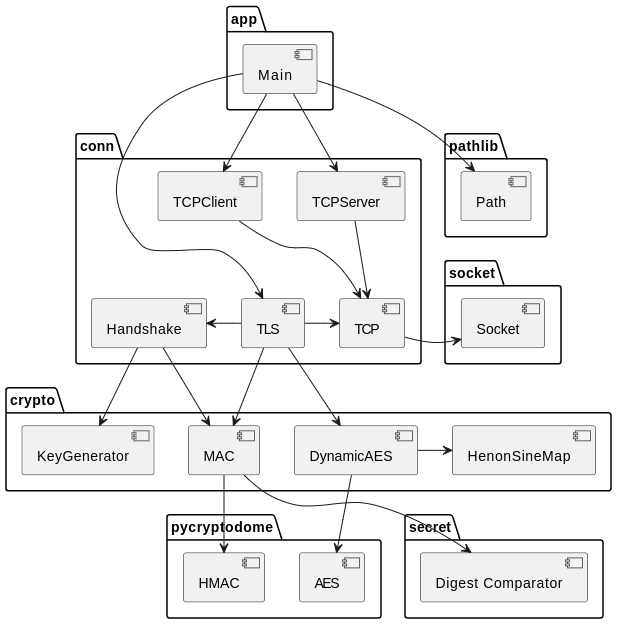
\includegraphics[width=0.9\textwidth]{chapters/res/chapter-4/impl.component.png}
  \caption{Diagram Komponen Implementasi Pustaka TLS Berbasis Sistem Chaos} \label{fig:impl.overview}
\end{figure}

Modul \texttt{main} merupakan \emph{entry point} dari aplikasi penguji dari pustaka yang dibangun. Pustaka terdiri atas beberapa modul penting, yaitu modul \texttt{data}, \texttt{conn}, dan \texttt{crypto}. Modul \texttt{data} digunakan untuk merepresentasikan data yang ada pada protokol TLS. Modul \texttt{conn} digunakan untuk mengatur komunikasi antara \emph{client} dan \emph{server}. Pada modul ini juga implementasi terkait protokol TLS dan TCP dibangun. Modul \texttt{crypto} digunakan untuk mengatur operasi kriptografi yang ada pada protokol TLS. 

Modul utilitas dan kriptografi digunakan untuk membantu dalam menyediakan fungsi-fungsi yang dapat membantu proses kriptografi, pembangkitan kunci, dan operasi lain yang dibutuhkan dalam proses pengembangan pustaka. Kelas yang ada pada modul ini dijelaskan pada tabel \ref{tab:impl.util}. Modul ini merupakan implementasi dari solusi S1, S2, S3, S4, S5, dan S6.

Tabel \ref{tab:impl.util} menjelaskan terkait fungsi utilitas yang diimplementasikan pada pustaka yang dibangun. Selain utilitas umum, terdapat beberapa kelas yang diimplementasikan sebagai utilitas yang memfasilitasi operasi kriptografi dan pembangkitan kunci acak. Tabel \ref{tab:impl.util.crypto} menjelaskan beberapa kelas yang diimplementasikan pada pustaka yang dibangun. 

Modul data digunakan untuk membantu dalam proses \emph{parsing} dan \emph{encode} data. Tabel \ref{tab:impl.data} menjelaskan beberapa kelas yang diimplementasikan pada pustaka yang dibangun. Semua kelas pada bagian ini terletak pada modul \texttt{data}. Tabel \ref{tab:impl.enum} menjelaskan beberapa enum yang diimplementasikan pada pustaka yang dibangun. Enum ini berisi beberapa konstanta yang digunakan pada protokol TLS.

Struktur data dari kelas yang diimplementasikan pada modul ini merupakan turunan dari struktur data yang didefinisikan pada \textcite{rfc5246} dan \textcite{rfc4492}. Struktur data lengkap yang menggambarkan implementasi pada penelitian ini dijelaskan pada Lampiran \ref{appendix:tls12.datatype}.

Modul \texttt{conn} bertanggung jawab dalam mengatur proses \emph{handshake}, proses komunikasi melalui TCP, komunikasi melalui UNIX Socket, serta proses enkripsi dan pengaturan \emph{state}. Tabel \ref{tab:impl.comm} menjelaskan beberapa kelas yang diimplementasikan pada pustaka yang dibangun. Semua kelas pada bagian ini terletak pada modul \texttt{conn}. Modul ini merupakan impelementasi dari solusi S3, S5, S7, S8, S9, dan S10.

\section{Pengujian}
Bagian ini menjelaskan dari pengujian yang dilakukan terhadap pustaka yang telah dibangun. Bagian ini akan menjelaskan terkait dengan detail pengujian yang dilakukan serta hasil dari pengujian tersebut.

\subsection{Tujuan Pengujian}
Pengujian dilakukan dengan tujuan sebagai berikut:
\begin{enumerate}
  \item Menguji fungsionalitas dan keamanan \emph{cipher} yang diusulkan.
  \item Menguji fungsionalitas dan keamanan implementasi protokol TLS yang dibangun.
\end{enumerate}

Pengujian fungsionalitas \emph{cipher} dilakukan untuk memastikan bahwa \emph{cipher} yang diusulkan dapat menjalankan proses kriptografi dengan baik. Pengujian ini dilakukan dengan melakukan operasi kriptografi pada \emph{cipher} sesuai dengan kasus yang didefinisikan. Pengujian keamanan pada \emph{cipher} dilakukan dengan melakukan uji statistik pada sistem \emph{chaos} dan \emph{cipher} yang diusulkan. Hal ini bertujuan untuk mengetahui sifat statistik yang mungkin muncul pada sistem \emph{chaos} dan hasil enkripsi dari \emph{cipher} yang diusulkan. Uji statistik dilakukan dengan menggunakan NIST Statistical Test Suite yang telah diimplementasikan oleh \textcite{marek2016}. Selain itu, pengujian keamanan juga dilakukan dengan menguji beberapa skenario serangan. Pengujian ini dilakukan untuk menguji jawaban atas rumusan masalah pertama.

\begin{table}[!h]
  \centering
  \caption{Lingkungan Pengujian} \label{tab:test.env}
  \begin{tabular}{|p{3cm}|p{6cm}|}
    \hline
    \textbf{Jenis Lingkungan} & \textbf{Nilai} \\ \hline
    Sistem Operasi & Fedora Linux 40 \\ \hline
    Kernel & Linux 6.8.9 \\ \hline
    Manager Paket & Pip 23.3.2 \\ \hline
    CPU & 11th Gen Intel i7-11800H (16) @ 4.600GHz \\ \hline
    RAM & 32GB \\ \hline
  \end{tabular}
\end{table}


Pengujian fungsionalitas protokol TLS dilakukan untuk memastikan bahwa protokol yang dibangun dapat berjalan dengan baik. Pengujian ini dilakukan dengan menggunakan skenario. Pengujian ini dilakukan secara \emph{end to end} testing. Pengujian keamanan protokol TLS dilakukan dengan menguji beberapa skenario serangan yang mungkin terjadi pada protokol TLS. Pengujian ini dilakukan untuk menguji jawaban atas rumusan masalah kedua.

\subsection{Lingkungan Pengujian}
Perangkat lunak dan pustaka yang digunakan pada pengujian ditunjukan pada tabel \ref{tab:test.lib}. Pengujian dilakukan pada perangkat dengan spesifikasi yang ditunjukan pada tabel \ref{tab:test.env}. 

Pengujian dilakukan pada sistem operasi linux ditujukan untuk menggunakan fitur dari \emph{UNIX socket} yang telah disediakan oleh kernel linux. Pemilihan \emph{UNIX socket} dilibatkan dalam pengujian ini dikarenakan fitur tersebut dapat mensimulasikan proses TCP tanpa perlu membuka port. Oleh karena itu, fitur ini dapat memudahkan pengujian khususnya bila menggunakan \emph{unit testing}.

\begin{table}[!h]
  \centering
  \caption{Pustaka Pengujian yang Digunakan} \label{tab:test.lib}
  \begin{tabular}{|p{4cm}|p{9cm}|}
    \hline
    \textbf{Nama Pustaka} & \textbf{Deskripsi} \\ \hline
    \texttt{pytest 8.1.1} & Pustaka ini digunakan untuk membantu dalam menyediakan \emph{runtime} pengujian dan membantu dalam proses \emph{debugging} bila terjadi kegagalan saat pengujian berlangsung. \\ \hline
    \texttt{socket} & Pustaka standard ini digunakan untuk melakukan komunikasi melalui \emph{UNIX socket}.\\ \hline
    \texttt{Fast Statictics Test v6.0.1} & Perangkat lunak ini digunakan dalam menguji keteracakan dari bytestream berdasarkan NIST Statistical Test Suite.\\ \hline
    \texttt{Wireshark} & Perangkat lunak ini digunakan dalam mengamati pesan \emph{ciphertext} yang dihasilkan oleh protokol komunikasi.\\ \hline
    \texttt{Python 3.12.3} & Perangkat lunak ini digunakan sebagai \emph{runtime} pustaka yang diuji.\\ \hline
    \end{tabular}
  \end{table}
    

  Pengujian statistik dilakukan dengan memanfaatkan Fast Statictics Test yang telah diimplementasikan oleh \textcite{marek2016}. Perangkat lunak ini merupakan optimasi dari implementasi pengujian perangkat lunak yang telah dibuat oleh NIST. Oleh karena itu, proses pengujian diharapkan dapat menjadi lebih cepat dan efisien. 

\subsection{Skenario dan Hasil Pengujian}

Bagian ini menjelaskan skenario pengujian yang dilakukan dan hasil dari pengujian yang telah disebutkan sebelumnya. Bagian ini dibagi menjadi dua bagian, yaitu pengujian \emph{cipher} dan pengujian implementasi protokol TLS.

\subsubsection{Pengujian \emph{Cipher}}

Pengujian \emph{cipher} dilakukan dengan dua tahap, yakni pengujian skenario dan pengujian statistik. Pengujian berbasis skenario dilakukan dengan beberapa skenario yang ditunjukan pada tabel \emph{test.case.cipher}. Pengujian statistik dilakukan dengan menggunakan Fast Statictics Test yang telah diimplementasikan oleh \textcite{marek2016}. Pengujian statistik ditujukan untuk menguji solusi S1 dan S4.

\begin{table}[!h]
  \centering
  \caption{Skenario Uji Cipher} \label{tab:test.case.cipher}
  \begin{tabular}{|c|p{7cm}|c|}
    \hline
    \textbf{Kode Kasus Uji} & \textbf{Deskripsi} & \textbf{ID Solusi Terkait} \\ \hline
    \multicolumn{3}{|l|}{Pengujian Fungsionalitas} \\ \hline
    T1.1 & \emph{Cipher} dapat melakukan proses enkripsi pada pesan teks rahasia dengan menggunakan cipher AES-256 kunci blok dinamis.  & S1, S4, dan S5\\ \hline
    T1.2 & \emph{Cipher} dapat mendekripsi kembali pesan menggunakan cipher AES-256 kunci blok dinamis. & S1, S4, dan S5\\ \hline
    \multicolumn{3}{|l|}{Pengujian Keamanan} \\ \hline
    T1.3 & Hasil dekripsi pada pesan yang dilakukan \emph{replay attack} haruslah gagal. & S1 dan S4\\ \hline
    T1.4 & Hasil enkripsi dari \emph{Cipher} pada dua blok yang memiliki pesan yang sama memiliki hasil blok yang berbeda. & S1 dan S4\\ \hline
  \end{tabular}
\end{table}

Pengujian skenario dilakukan dengan menggunakan \emph{unit testing} yang telah diimplementasikan pada pustaka yang dibangun. Pengujian ini dilakukan dengan menggunakan pustaka \texttt{pytest} yang telah dijelaskan pada bagian sebelumnya. Pengujian ini dilakukan dengan menggunakan skenario yang telah dijelaskan pada tabel \ref{tab:test.case.cipher}. Pengujian skenario dikatakan berhasil apabila semua skenario yang telah dijalankan mendapatkan hasil \emph{pass}.

Pengujian statistik pada dasarnya dilakukan dengan menguji keteracakan dari bytestream yang dihasilkan oleh sistem \emph{chaos} dan \emph{cipher}. Alasan dilakukannya pengujian keteracakan pada \emph{cipher} adalah memastikan bahwa cipher tidak memiliki pola-pola statistik yang memungkinkan melemahkan \emph{cipher} yang digunakan. Hasil dari pengujian statistik akan dibandingkan dengan acuan yang dipilih. Uji statistik ini berhasil apabila kualitas dari bytestream yang dihasilkan oleh sistem \emph{chaos} dan \emph{cipher} memiliki kualitas yang setara atau lebih baik dengan acuan yang dipilih. Kualitas ditentukan berdasarkan proporsi \emph{pass} dari uji statistik yang dilakukan. Pengujian kesetaraan dilakukan dengan uji hipotesis perbandingan proporsi dengan \emph{confidence level} sebesar 95\%.

Acuan yang digunakan untuk menilai kualitas dari keteracakan sistem \emph{chaos} adalah sistem acak \texttt{/dev/urandom} yang ada pada sistem linux. Acuan ini dipilih dikarenakan sistem acak \texttt{urandom} termasuk sistem acak aman yang sering digunakan dalam proses kriptografi. 

Acuan yang digunakan untuk menilai kualitas dari keteracakan \emph{cipher} adalah \emph{cipher} AES-256 kunci blok statis dengan blok CTR yang ada pada pustaka \texttt{pycryptodome}. Pemilihan acuan ini dikarenakan AES-256 kunci blok statis dengan blok CTR merupakan \emph{cipher} yang setara dengan implementasi \emph{cipher} yang diusulkan pada penelitian ini.

Hasil dari pengujian skenario ditunjukan pada tabel \ref{tab:test.result.cipher}. Hasil tersebut menunjukan bahwa semua syarat yang dijalankan terpenuhi. Bukti serta algoritma dari pengujian ini dapat dilihat pada lampiran \ref{appendix:unit.test.cipher}. Oleh karena itu, dapat disimpulkan bahwa \emph{cipher} yang diusulkan dapat berjalan dengan baik pada skenario yang telah dijalankan.

\begin{table}[!h]
  \centering
  \caption{Hasil Pengujian Cipher dengan Metode Skenario} \label{tab:test.result.cipher}
  \begin{tabular}{|c|c|}
    \hline
    \textbf{Kode Kasus Uji} & \textbf{Hasil} \\ \hline
    T1.1 & Berhasil \\ \hline
    T1.2 & Berhasil \\ \hline
    T1.3 & Berhasil \\ \hline
    T1.4 & Berhasil \\ \hline
  \end{tabular}
\end{table}

Pengujian statistik CSPRNG dilakukan dengan membandingkan proporsi \emph{pass} pada CSPRNG berbasis Sine-Henon dan CSPRNG berbasis \texttt{/dev/urandom}. Hipotesis nol ($\text{H}_0$) yang dipilih dalam pengujian ini adalah proporsi \emph{pass} CSPRNG berbasis sistem \emph{chaos} Sine-Henon map sama dengan atau lebih besar dari proporsi \emph{pass} dari CSPRNG \texttt{/dev/urandom}. Hipotesis alternatif ($\text{H}_1$) yang dipilih adalah proporsi \emph{pass} dari Sine-Henon map lebih kecil dari proporsi \emph{pass} dari \texttt{/dev/urandom}. Nilai titik kritis dari pengujian ini adalah -1.64.

\begin{table}[!h]
  \centering
  \caption{Hasil Pengujian Statistik pada CSPRNG Berbasis Sistem \emph{Chaos} Sine-Henon Map dan \texttt{/dev/urandom}} \label{tab:test.statistic.chaos}
  \begin{tabular}{|c|c|c|c|}
    \hline
    \textbf{Nama Pengujian }& \textbf{\texttt{/dev/urandom}} & \textbf{Sine-Henon Map} & \textbf{P-Value} \\ \hline
    Uji Entropi & 98,8\% & 99\% & 0,000606 \\ \hline
    Uji Frekuensi Blok & 99,2\% & 99,2\% & 0,000000 \\ \hline
    Uji Jumlah Kumulatif & 98,9\% & 99,7\% & 0,003034 \\ \hline
    Uji FFT & 98,8\% & 97,2\% & -0.003614 \\ \hline
    Uji Frekuensi & 98,4\% & 99,6\% & 0,003814 \\ \hline
    Uji Kompleksitas Linear & 98,0\% & 99,0\% & 0,002602 \\ \hline
    Uji \emph{Runs} terpanjang & 99,6\% & 98,2\% & -0,004245 \\ \hline
    Uji \emph{Non Overlapping Template} & 98,9\% & 98,2\% & -0,000193 \\ \hline
    Uji \emph{Overlapping Template} & 99,0\% & 99,0\% & 0,000000 \\ \hline
    Uji \emph{Random Excursions} & 98,6\% & 99,3\% & 0,002257 \\ \hline
    Uji \emph{Random Excursions Variant} & 98,8\% & 98,8\% & -0,000245 \\ \hline
    Uji Rank & 99,4\% & 99,4\% & 0,000000 \\ \hline
    Uji \emph{Runs} & 99,2\% & 99,2\% & 0,000000 \\ \hline
    Uji Serial & 99,3\% & 98,7\% & -0,001907 \\ \hline
    Uji Universal & 98,6\% & 99,0\% & 0,001162 \\ \hline
  \end{tabular}
\end{table}

Hasil dari pengujian statistik pada \emph{cipher} ditunjukan pada tabel \ref{tab:test.statistic.chaos}. Nilai P-value pada tabel tersebut menunjukan nilai yang lebih besar dari nilai titik kritis yang dipilih. Oleh karena itu, hipotesis nol ($\text{H}_0$) dapat diterima. Oleh karena itu, dapat disimpulkan bahwa CSPRNG berbasis sistem \emph{chaos} Sine-Henon map yang dibangun memiliki kualitas keteracakan yang setara dengan sistem random \texttt{/dev/urandom}.

Pengujian statistik pada \emph{cipher} dilakukan dengan membandingkan proporsi \emph{pass} pada \emph{cipher} berbasis AES-256 kunci blok dinamis dan \emph{cipher} berbasis AES-256 kunci blok statis dengan mode blok yang sama. Hipotesis nol ($\text{H}_0$) yang dipilih dalam pengujian ini adalah proporsi \emph{pass} dari \emph{cipher} berbasis AES-256 kunci blok dinamis sama dengan atau lebih besar dari proporsi \emph{pass} dari \emph{cipher} berbasis AES-256 kunci blok statis. Hipotesis alternatif ($\text{H}_1$) yang dipilih adalah proporsi \emph{pass} dari \emph{cipher} berbasis AES-256 kunci blok dinamis lebih kecil dari proporsi \emph{pass} dari \emph{cipher} berbasis AES-256 kunci statis. Nilai titik kritis dari pengujian ini adalah -1.64. Nilai ini diambil berdasarkan uji hipotesis perbandingan proporsi dengan \emph{confidence level} sebesar 95\%.

\begin{table}[!h]
  \centering
  \caption{Hasil Pengujian Statistik pada Cipher Blok Statis dan Blok Dinamis} \label{tab:test.statistic.cipher}
  \begin{tabular}{|c|c|c|c|}
    \hline
    \textbf{Nama Pengujian} & \textbf{Blok Statis} & \textbf{Blok Dinamis} & \textbf{P-Value} \\ \hline
    Uji Entropi & 98,6\% & 98,2\% & -0,504049 \\ \hline
    Uji Frekuensi Blok & 99,0\% & 98,4\% & 0,837512 \\ \hline
    Uji Jumlah Kumulatif & 98,5\% & 99,2\% & 1.038080 \\ \hline
    Uji FFT & 98,0\% & 98,4\% & 0,475705 \\ \hline
    Uji Frekuensi & 98,6\% & 99,2\% & 0,909550 \\ \hline
    Uji Kompleksitas Linear & 99,0\% & 99,2\% & 0,334844 \\ \hline
    Uji \emph{Runs} terpanjang & 99,2\% & 99,0\% & -0,334844 \\ \hline
    Uji \emph{Non Overlapping Template} & 99,0\% & 99,0\% & -0,037565 \\ \hline
    Uji \emph{Overlapping Template} & 99,2\% & 98,8\% & -0,635642 \\ \hline
    Uji \emph{Random Excursions} & 98,1\% & 98,6\% & -0,787570 \\ \hline
    Uji \emph{Random Excursions Variant} & 98,8\% & 99,2\% & 0,607298 \\ \hline
    Uji Rank & 99,4\% & 98,8\% & -1.004531 \\ \hline
    Uji \emph{Runs} & 98,8\% & 99,1\% & 1.674218 \\ \hline
    Uji Serial & 99,2\% & 99,0\% & 0,635642 \\ \hline
    Uji Universal & 99,4\% & 99,4\% & 0,000000 \\ \hline
  \end{tabular}
\end{table}

Hasil dari pengujian statistik pada \emph{cipher} ditunjukan pada tabel \ref{tab:test.statistic.cipher}. Nilai P-value pada tabel tersebut menunjukan nilai yang lebih besar dari nilai titik kritis yang dipilih. Oleh karena itu, hipotesis nol ($\text{H}_0$) dapat diterima. Oleh karena itu, dapat disimpulkan bahwa \emph{cipher} yang diusulkan memiliki kualitas keteracakan yang setara dengan \emph{cipher} AES-256 kunci blok statis.

\subsubsection{Pengujian Implementasi Protokol TLS}

Pengujian implementasi protokol TLS dan integrasi dengan \emph{cipher} AES kunci blok dinamis dilakukan dengan pengujian skenario. Pengujian ini dilakukan secara \emph{end-to-end}. Pengujian ini dilakukan dengan tujuan untuk menguji fungsionalitas dan keamanan dari protokol TLS yang dibangun. Pengujian ini dikatakan berhasil apabila telah memenuhi semua skenario yang telah dijalankan. Skenario pengujian ditunjukan pada tabel \ref{tab:test.case.tls}.

\begin{table}[!h]
  \centering
  \caption{Skenario Uji Implementasi Protokol TLS} \label{tab:test.case.tls}
  \begin{tabular}{|c|p{7cm}|p{3cm}|}
    \hline
    \textbf{Kode Kasus Uji} & \textbf{Deskripsi} & \textbf{ID Solusi Terkait} \\ \hline
    \multicolumn{3}{|l|}{Pengujian Fungsionalitas} \\ \hline
    T2.1 & Protokol TLS dapat melakukan proses \emph{handshake} dan membentuk sistem \emph{chaos} yang sesuai pada tiap-tiap partisipan. & S2, S3, S7, S8, dan S9\\ \hline
    T2.2 & Protokol TLS dapat digunakan untuk mengirim dan menerima pesan teks. & S1, S4, S5, S6, dan S9 \\ \hline
    T2.3 & Protokol TLS dapat digunakan untuk mengirim dan menerima pesan biner. & S1, S4, S5, S6, dan S9 \\ \hline
    \multicolumn{3}{|l|}{Pengujian Keamanan} \\ \hline
    T2.4 & Protokol TLS dapat menangani kasus \emph{tampering} pada parameter ECDH. & S8 dan S9 \\ \hline
    T2.5 & Protokol TLS dapat menangani kasus kunci privat yang salah saat menandatangani parameter ECDH.  & S7, S8, dan S9 \\ \hline
    T2.6 & Protokol TLS dapat menangani kasus MAC yang tidak valid. & S6 dan S9 \\ \hline
    T2.7 & Protokol TLS masih dapat menerima pesan setelah mendapatkan \emph{frame} dengan MAC yang tidak valid.  & S5, S6, dan S9 \\ \hline
    T2.8 & Protokol TLS dapat menangani kasus \emph{replay attack} pada saat koneksi telah terjalin. & S5, S6, dan S9 \\ \hline
    T2.9 & Protokol TLS masih dapat menerima pesan setelah mendapatkan serangan \emph{replay}. & S5, S6, dan S9 \\ \hline
    T2.10 & Frame terenkripsi yang dihasilkan oleh protokol ini harus memiliki \emph{ciphertext} yang berbeda pada \emph{plaintext} yang sama. & S4 dan S5 \\ \hline
    T2.11 & Protokol TLS dapat menangani kasus \emph{tampering} pada pesan Client Hello. & S9 \\ \hline
    T2.12 & Protokol TLS dapat menangani kasus \emph{tampering} pada pesan Server Hello. & S9 \\ \hline
    T2.13 & Protokol TLS dapat menangani kasus \emph{certificate} server yang tidak sesuai dengan \emph{certificate pinning} pada \emph{client}.  & S9 dan S10 \\ \hline
  \end{tabular}
\end{table}


Pengujian skenario dilakukan dengan menggunakan \emph{unit testing} yang telah diimplementasikan pada pustaka yang dibangun. Pengujian ini dilakukan dengan menggunakan pustaka \texttt{pytest} yang telah dijelaskan pada bagian sebelumnya. Detail implementasi dan bukti dari pengujian ini dijelaskan pada Lampiran \ref{appendix:unit.test.tls}. Hasil pengujian skenario ditunjukan pada tabel \ref{tab:test.result.tls}

\begin{table}[!h]
  \centering
  \caption{Hasil Pengujian Implementasi TLS} \label{tab:test.result.tls}
  \begin{tabular}{|c|c|}
    \hline
    \textbf{Kode Kasus Uji} & \textbf{Hasil} \\ \hline
    T2.1 & Berhasil \\ \hline
    T2.2 & Berhasil \\ \hline
    T2.3 & Berhasil \\ \hline
    T2.4 & Berhasil \\ \hline
    T2.5 & Berhasil \\ \hline
    T2.6 & Berhasil \\ \hline
    T2.7 & Berhasil \\ \hline
    T2.8 & Berhasil \\ \hline
    T2.9 & Berhasil \\ \hline
    T2.10 & Berhasil \\ \hline
    T2.11 & Berhasil \\ \hline
    T2.12 & Berhasil \\ \hline
    T2.13 & Berhasil \\ \hline
  \end{tabular}
\end{table}

\section{Analisis Hasil Pengujian} 
\label{sec:analisis-hasil-pengujian}

Bagian ini akan membahas terkait hasil pengujian serta ancaman validitas dari hasil pengujian yang telah dilakukan. Bagian ini akan terbagi menjadi analisis hasil pengujian untuk \emph{cipher} dan analisis hasil pengujian untuk implementasi protokol TLS.

\subsection{Analisis Hasil Pengujian \emph{Cipher}}

Pengujian berbasis skenario memiliki dua kelompok pengujian. Kelompok pertama adalah pengujian fungsionalitas yang dilakukan dengan skenario T1.1 dan T1.2. Kelompok kedua adalah pengujian keamanan berbasis skenario yang dilakukan pada skenario T1.3 dan T1.4. Hasil kedua kelompok pengujian tersebut menunjukan bahwa \emph{cipher} AES blok dinamis berbasis sistem \emph{chaos} Sine-Henon map dapat bekerja dengan baik baik pada keamanan maupun fungsionalitas.

Pengujian statistik yang dilakukan pada CSPRNG menunjukan bahwa sistem random berbasis Sine-Henon map memiliki kualitas keteracakan yang setara dengan sistem random \texttt{/dev/urandom}. Selain itu, pengujian statistik yang dilakukan pada \emph{cipher} AES-256 kunci blok dinamis menunjukan bahwa \emph{cipher} yang diusulkan memiliki kualitas keteracakan yang setara dengan \emph{cipher} AES-256 kunci blok statis. Oleh karena itu, kualitas keamanan dari \emph{cipher} yang diusulkan dapat dikatakan setara dengan \emph{cipher} AES-256 kunci blok statis.

Berdasarkan kedua pengujian tersebut, enkripsi dengan menggunakan AES kunci blok dinamis berbasis sistem \emph{chaos} Sine-Henon map dapat digunakan sebagai \emph{cipher} yang aman dan fungsional. Metode enkripsi ini dapat digunakan dalam melakukan enkripsi pesan rahasia. Oleh karena itu, dapat disimpulkan bahwa rumusan masalah pertama dapat terjawab dengan menggunakan sistem \emph{chaos} Sine-Henon map sebagai CSPRNG penghasil kunci blok dinamis.

\subsection{Analisis Hasil Pengujian Implementasi Protokol TLS}

Pengujian implementasi protokol TLS menunjukan bahwa pengujian keamanan serta pengujian fungsionalitas dapat berjalan dengan baik. Pengujian keamanan yang dilakukan pada protokol TLS menunjukan bahwa protokol TLS yang dibangun dapat menangani \emph{replay attack}, serangan \emph{tampering}, serta serangan MITM.  Pengujian fungsionalitas yang dilakukan pada protokol TLS menunjukan bahwa protokol TLS yang dibangun dapat melakukan proses \emph{handshake}, enkripsi pesan, serta dekripsi pesan dengan baik. Oleh karena itu, dapat disimpulkan bahwa protokol TLS yang dibangun dapat digunakan sebagai protokol komunikasi yang aman dan fungsional.

Berdasarkan hasil pengujian tersebut, dapat disimpulkan bahwa \emph{cipher} AES kunci blok dinamis berbasis sistem \emph{chaos} Sine-Henon map dapat digunakan sebagai \emph{cipher} pada protokol TLS. Hal ini dikarenakan \emph{cipher} yang diusulkan dapat berjalan dengan baik pada protokol TLS yang dibangun. Oleh karena itu, dapat disimpulkan bahwa rumusan masalah kedua dapat terjawab dengan menggunakan \emph{cipher} AES kunci blok dinamis berbasis sistem \emph{chaos} Sine-Henon map dengan mengikuti protokol TLSv1.2 dan penyesuaian sebagaimana yang telah dijelaskan pada bagian \ref{sec:protokol-tls-chaos}.

\subsection{Ancaman Validitas (Threat of Validity)}

Pengujian yang dilakukan memiliki beberapa ancaman validitas yang perlu diperhatikan. Hal ini dikarenakan terdapat beberapa asumsi yang diambil dalam menguji protokol ini. Asumsi yang diambil dalam pengujian ini adalah sebagai berikut:
\begin{enumerate}
  \item Pengujian mengasumsikan bahwa protokol TLS telah teruji keamanannya, sehingga serangan selain yang berkaitan dengan pembentukan \emph{cipher} dan \emph{ciphertext} tidak diuji.
  \item Pengujian mengasumsikan bahwa \emph{cipher} AES tahan terhadap serangan \emph{brute-force} dan \emph{side-channel} sehingga metode serangan tersebut tidak diuji.
  \item Proses serangan MITM diasumsikan dilakukan dengan mengganti sertifikat digital yang digunakan pada protokol TLS.
  \item Serangan \emph{tampering} hanya dilakukan pada \emph{frame} yang berkaitan dengan pembentukan \emph{cipher} dan \emph{ciphertext}. Hal ini bertujuan agar dapat mengubah atau membaca pesan yang dikirimkan.
  \item Serangan \emph{side-channel} yang dilakukan diasumsikan dilakukan dengan mengamati pola \emph{ciphertext} yang dihasilkan oleh protokol TLS.
\end{enumerate}

% \chapter{Kesimpulan dan Saran}

\section{Kesimpulan}
Berdasarkan hasil analisis, implementasi, dan pengujian yang telah dilakukan, diperoleh kesimpulan sebagai berikut:
\begin{enumerate}
  \item Proses enkripsi pesan memanfaatkan Algoritme AES kunci blok dinamis yang aman dapat dilakukan dengan melibatkan CSPRNG berbasis \emph{chaos} pada pembangkitan kunci blok. Salah satu sistem \emph{chaos} yang cukup baik adalah Sine-Henon Map. Mode blok yang dapat digunakan pada \emph{cipher} adalah CTR. Enkripsi dilakukan dengan membagi pesan menjadi beberapa blok, selanjutnya blok tersebut dienkripsi dengan kunci blok yang dihasilkan dari \emph{chaos} dan counter yang dihasilkan dari \emph{chaos}. Proses dekripsi dilakukan dengan cara membentuk kunci dan counter menggunakan \emph{chaos}. Algoritme ini memiliki kualitas keamanan yang baik berdasarkan Uji Statistik NIST dan Skenario serangan \emph{replay}.
  \item Pengimplementasian Algoritme AES kunci blok dinamis pada berbasis sistem \emph{chaos} dapat dilakukan pada protokol TLSv1.2. Proses implementasi dilakukan dengan membuat sebuah \emph{cipher suite} pada protokol TLSv1.2. Sebelum melakukan proses enkripsi dan dekripsi, sistem harus menyimpan nilai \emph{state} awal dari sistem \emph{chaos}. Hal ini ditujukan agar bila terjadi kegagalan pada proses enkripsi dan dekripsi, sistem dapat mengembalikan nilai \emph{state} sistem \emph{chaos} ke posisi yang semula. Hasil pengujian menunjukkan bahwa protokol yang dibangun dapat berjalan dengan baik. Berdasarkan pengujian, Protokol ini mampu tahan terhadap serangan \emph{replay}, serangan analisis \emph{ciphertext}, dan serangan \emph{tampering}.
\end{enumerate}

\section{Saran}
Adapun saran terkait pelaksanaan Tugas Akhir ini adalah sebagai berikut:
\begin{enumerate}
  \item Optimasi yang dilakukan pada pembangkitan nilai \emph{chaos} yang digunakan pada pembangkitan kunci blok.
  \item Penerapan proses paralelisasi saat melakukan proses enkripsi dan dekripsi.
  \item Implementasi \emph{cipher} AES dinamis pada protokol TLSv1.3. 
\end{enumerate}
%----------------------------------------------------------------%

% Daftar pustaka
\printbibliography
% \blankpage

% Setting judul lampiran
\titlespacing*{\chapter}{0pt}{0pt}{0pt}
\titlespacing*{\section}{0pt}{0pt}{*1}

% Setting judul anak lampiran
\titleformat*{\section}{\bfseries}

% Index
\appendix
\chapter{{{Tipe Data Protokol TLSv1.2}}} 
\label{appendix:tls12.datatype}

Berikut ini merupakan daftar dari tipe data yang digunakan pada protokol TLSv1.2. Daftar ini diimplementasikan pada \textcite{rfc5246} dan \textcite{rfc4492}.

\section{Layer \emph{Record}}

\begin{verbatim}
  struct {
    uint8 major;
    uint8 minor;
  } ProtocolVersion;

  ProtocolVersion version = { 3, 3 }; /* TLS v1.2*/

  enum {
      change_cipher_spec(20), alert(21), handshake(22),
      application_data(23), (255)
  } ContentType;

  struct {
      ContentType type;
      ProtocolVersion version;
      uint16 length;
      opaque fragment[TLSPlaintext.length];
  } TLSPlaintext;

  struct {
    ContentType type;
    ProtocolVersion version;
    uint16 length;
    select (SecurityParameters.cipher_type) {
        case stream: GenericStreamCipher;
        case block:  GenericBlockCipher;
        case aead:   GenericAEADCipher;
    } fragment;
  } TLSCiphertext;

\end{verbatim}

\section{\emph{Change Cipher Spec}}

\begin{verbatim}
  struct {
       enum { change_cipher_spec(1), (255) } type;
   } ChangeCipherSpec;
\end{verbatim}

\section{Protokol \emph{Handshake}}

\begin{verbatim}
  enum {
    hello_request(0), client_hello(1), server_hello(2),
    certificate(11), server_key_exchange (12),
    certificate_request(13), server_hello_done(14),
    certificate_verify(15), client_key_exchange(16),
    finished(20)
    (255)
} HandshakeType;

struct {
    HandshakeType msg_type;
    uint24 length;
    select (HandshakeType) {
        case hello_request:       HelloRequest;
        case client_hello:        ClientHello;
        case server_hello:        ServerHello;
        case certificate:         Certificate;
        case server_key_exchange: ServerKeyExchange;
        case certificate_request: CertificateRequest;
        case server_hello_done:   ServerHelloDone;
        case certificate_verify:  CertificateVerify;
        case client_key_exchange: ClientKeyExchange;
        case finished:            Finished;
    } body;
} Handshake;

\end{verbatim}

\section{Pesan Hello}

\begin{verbatim}
  struct { } HelloRequest;

  struct {
      uint32 gmt_unix_time;
      opaque random_bytes[28];
  } Random;

  opaque SessionID<0..32>;

  uint8 CipherSuite[2];

  enum { null(0), (255) } CompressionMethod;

  struct {
      ProtocolVersion client_version;
      Random random;
      SessionID session_id;
      CipherSuite cipher_suites<2..2^16-2>;
      CompressionMethod compression_methods<1..2^8-1>;
      select (extensions_present) {
          case false:
              struct {};
          case true:
              Extension extensions<0..2^16-1>;
      };
  } ClientHello;

  struct {
      ProtocolVersion server_version;
      Random random;
      SessionID session_id;
      CipherSuite cipher_suite;
      CompressionMethod compression_method;
      select (extensions_present) {
          case false:
              struct {};
          case true:
              Extension extensions<0..2^16-1>;
      };
  } ServerHello;

  enum{
    none(0), md5(1), sha1(2), sha224(3), sha256(4), sha384(5),
    sha512(6), (255)
  } HashAlgorithm;

  enum {
    anonymous(0), rsa(1), dsa(2), ecdsa(3), (255)
  } SignatureAlgorithm;

  struct {
        HashAlgorithm hash;
        SignatureAlgorithm signature;
  } SignatureAndHashAlgorithm;

  SignatureAndHashAlgorithm
  supported_signature_algorithms<2..2^16-1>;
\end{verbatim}

\section{Otentikasi Server dan Pesan Pertukaran Kunci}

\begin{verbatim}
  opaque ASN.1Cert<2^24-1>;

  struct {
      ASN.1Cert certificate_list<0..2^24-1>;
  } Certificate;

  enum { dhe_dss, dhe_rsa, dh_anon, rsa,dh_dss, dh_rsa, ec_diffie_hellman
       } KeyExchangeAlgorithm;

  struct {
      opaque dh_p<1..2^16-1>;
      opaque dh_g<1..2^16-1>;
      opaque dh_Ys<1..2^16-1>;
  } ServerDHParams;     /* Ephemeral DH parameters */

  struct {
    select (KeyExchangeAlgorithm) {
        case dh_anon:
            ServerDHParams params;
        case dhe_dss:
        case dhe_rsa:
            ServerDHParams params;
            digitally-signed struct {
                opaque client_random[32];
                opaque server_random[32];
                ServerDHParams params;
            } signed_params;
        case rsa:
        case dh_dss:
        case dh_rsa:
            struct {} ;
        case ec_diffie_hellman:
            ServerECDHParams    params;
            Signature           signed_params;
    }
  } ServerKeyExchange;

  enum {
      rsa_sign(1), dss_sign(2), rsa_fixed_dh(3), dss_fixed_dh(4),
      rsa_ephemeral_dh_RESERVED(5), dss_ephemeral_dh_RESERVED(6),
      fortezza_dms_RESERVED(20),
      (255)
  } ClientCertificateType;

  struct { } ServerHelloDone;

  enum {
    deprecated(1..22),
    secp256r1 (23), secp384r1 (24), secp521r1 (25),
    x25519(29), x448(30),
    reserved (0xFE00..0xFEFF),
    deprecated(0xFF01..0xFF02),
    (0xFFFF)
  } NamedCurve;

  enum {
    deprecated (1..2),
    named_curve (3),
    reserved(248..255)
  } ECCurveType;


  struct {
    opaque point <1..2^8-1>;
  } ECPoint;

  struct {
    ECCurveType    curve_type;
    select (curve_type) {
        case named_curve:
            NamedCurve namedcurve;
    };
  } ECParameters;

  struct {
    ECParameters    curve_params;
    ECPoint         public;
  } ServerECDHParams;

  enum {
    ecdsa(3),
    ed25519(7)
    ed448(8)
  } SignatureAlgorithm;

  select (SignatureAlgorithm) {
   case ecdsa:
        digitally-signed struct {
            opaque sha_hash[sha_size];
        };
   case ed25519,ed448:
        digitally-signed struct {
            opaque rawdata[rawdata_size];
        };
  } Signature;

  /* Rumus Perhitungan Tanda Tangan Digital */
  ServerKeyExchange.signed_params.sha_hash
  SHA(ClientHello.random + ServerHello.random +
                         ServerKeyExchange.params);
  ServerKeyExchange.signed_params.rawdata
  ClientHello.random + ServerHello.random +
                         ServerKeyExchange.params;

\end{verbatim}

\section{Otentikasi Klien dan Pertukaran Kunci}

\begin{verbatim}
  struct {
    select (KeyExchangeAlgorithm) {
        case rsa:
            EncryptedPreMasterSecret;
        case dhe_dss:
        case dhe_rsa:
        case dh_dss:
        case dh_rsa:
        case dh_anon:
            ClientDiffieHellmanPublic;
    } exchange_keys;
  } ClientKeyExchange;

  enum { implicit, explicit } PublicValueEncoding;

  struct {
      select (PublicValueEncoding) {
          case implicit: struct {};
          case explicit: opaque DH_Yc<1..2^16-1>;
      } dh_public;
  } ClientDiffieHellmanPublic;


\end{verbatim}

\end{document}
